\documentclass[../structure.tex]{subfiles}
\begin{document}
\chapter{Results}
\hspace{2em}After implementing non-rigid ICP, we test the tools we have developed to assess the algorithm. We use data collected from \textbf{\textit{Human Connectome Projects}} \cite{CCF}. The number of samples used for testing is four with eleven pathways (bundles) in each side of the brain. We present two experiments to show how the method works from the same patient. The first experiment is left and right side of the same pathway and the second one is for one pathway, which deformed and re-registered again with the original shape.

% Statistic
\begin{center}
\begin{table}[h!]
	\begin{tabular}{| c | c  c  c | c  c  c |}
	%\begin{tabular}{*7c}
	\toprule
	&\multicolumn{3}{c}{Tracts}&\multicolumn{3}{c}{Points}\\
Pathways&Average&Max&Min&Average&Max&Min\\
\midrule
%\hline
ATR&266.75&603&106&26443.875&69283&9623\\
rostrum&1853.375&2020&1633&162936.625&188143&137536\\
Cing&1103.375&1369&872&167488.25&244088&100762\\
CST&1649.25&2044&1476&235265.375&308769&170535\\
Fornix&399&497&308&26618&37142&16703\\
genu&2134.5&2333&1967&166567.625&236384&144492\\
IFOF&862.875&985&774&128850.875&162086&90424\\
ILF&3751&4392&2950&566332.25&673060&367155\\
SLF&1333.125&1633&1044&174943.5&251994&105245\\
splenium&2209.625&2335&2063&206526.875&244341&182993\\
VTA&327.625&679&150&27784.125&54904&14982\\
\bottomrule
	\end{tabular}
\caption{The statistics of tracts (streamlines) and points in data}
\label{table:data}
\end{table}
\end{center}

\section{DIPY registration Method}
We compare our tools with a registration method discussed in \cite{Garyfallidis2015} and implemented in \textit{DIPY} package.

The method starts by reducing the number of points in each tract to a certain number of point, which is necessary for the method to have the same number of points in each tract.

DIPY method gets the initial orientation by placing both bundles (streamlines) in the origin point of the 3D Euclidean space. In this case, it considers only translation but not other transformations. To solve this problem and to be fare on the comparison, we use PCA tool that we develop to get the initial alignment before applying the DIPY method.

DIPY calculate the distance between template bundle and target bundle using a function called \textit{minimum average direct-flip distance (MDF)}. MDF is asymmetric
distance function, which can be applied only when all tracts have the same number of points, that is one reason why we reduce the number of point before applying DIPY registration, another reason is increasing the speed of distance calculation \cite{Garyfallidis2012}.

The method then uses optimizer to select the best combination of variables, which later converted to affine matrix, while reducing the overall distance between template bundle.

\begin{comment}
\section{ICP testing steps}
\begin{itemize}
\item Read bundles from \textit{ply} files
\item Save the visual orientation of the original alignment
\item Apply PCA
\item Visualize bundles after PCA and compare with original visual orientation
\item If the visual inspection was positive and PCA improved the alignment, we consider its result, otherwise we just flip the template bundle or consider the original orientation
\item Generate distances histogram between two bundles to select the distance threshold
\item Start the registration and iterate until there is no more improvement on the alignment
\end{itemize}
\end{comment}

\section{Experiment (1)}
\hspace{2em}In this experiment we use both side of Thalamic Radiation (ATR) fiber pathway, whereas the template bundle is the ATR on the right side and the target bundle is the left side of the ATR from the same patient.

First, we read the data (left and right side of ATR) using a tool that we customized from \textit{PlyFile} package to suit our data. Then we apply PCA and visually inspect the result as shown in Figures \ref{fig:img_original} and \ref{fig:img_PCA}. If PCA improves the alignment, we consider its alignment, otherwise we accept the original orientation if it sufficient or just flip the template bundle if two bundles are from different side of the brain.

\begin{figure}[h!]
\centering
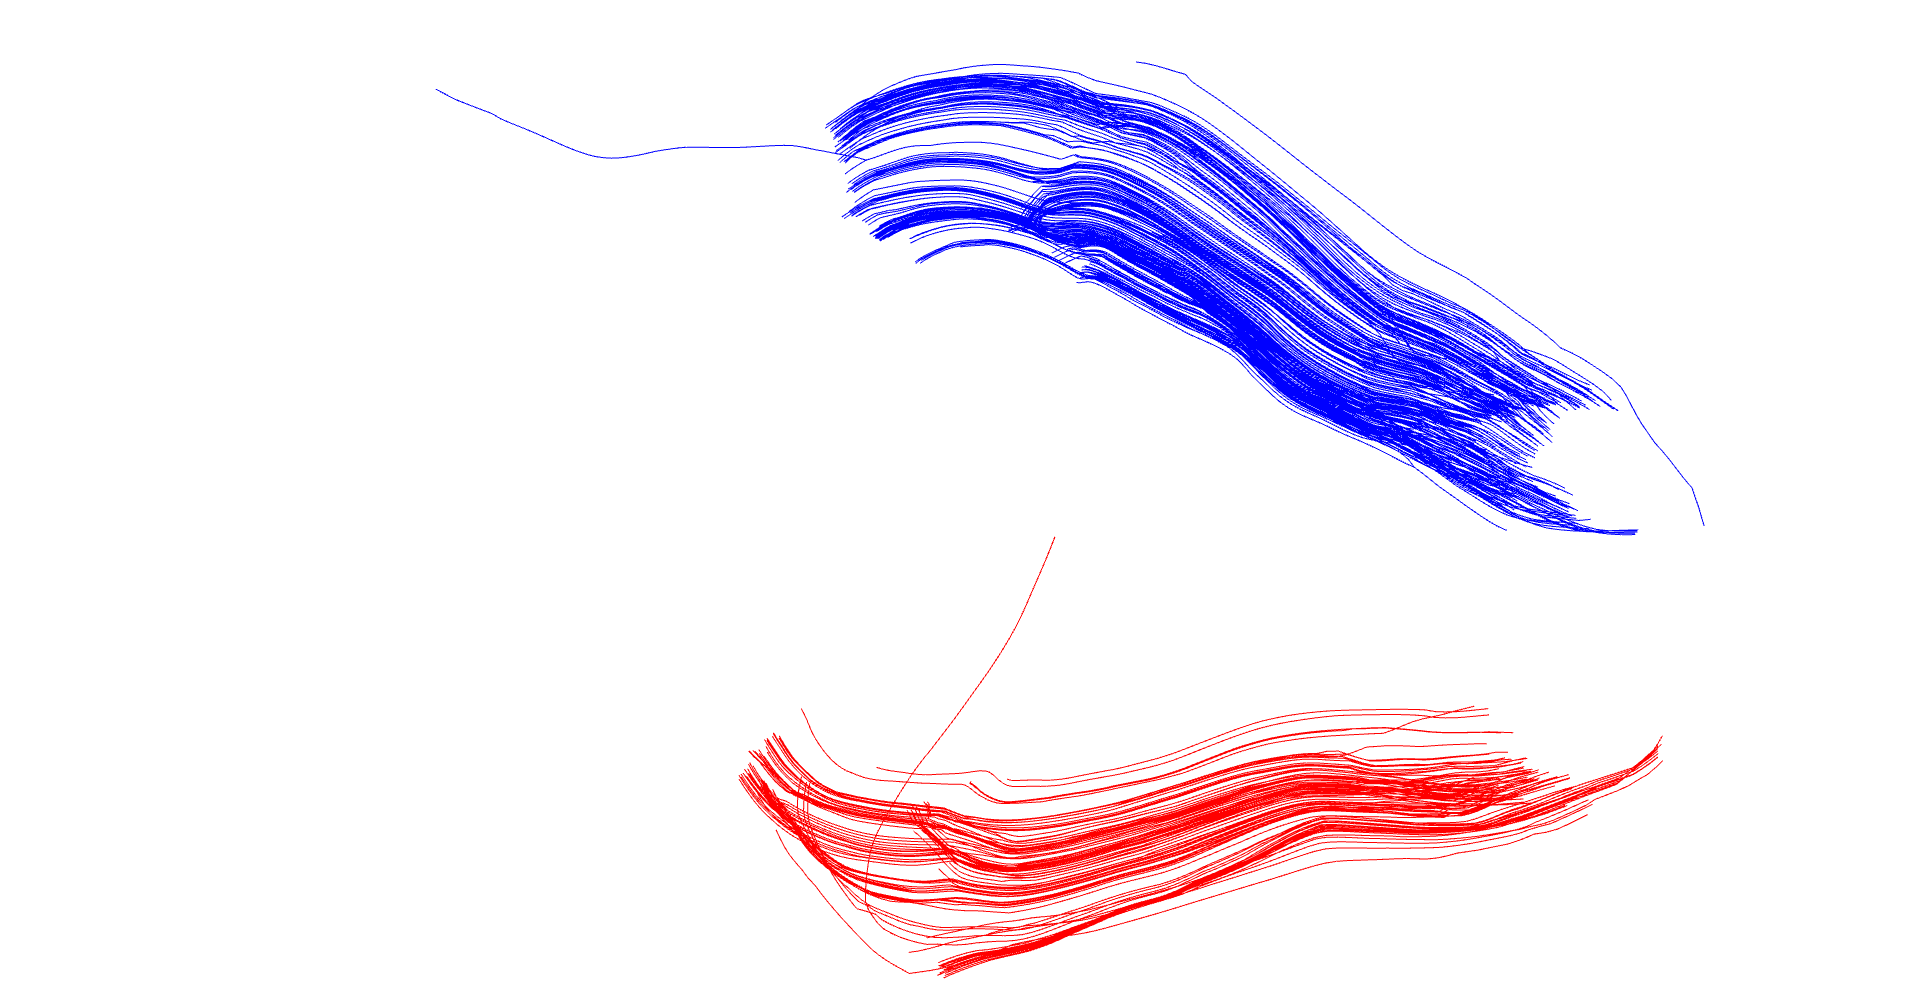
\includegraphics[scale=.8]{101_img_original}
\captionsetup{justification=centering}
\caption{The original orientation of ATR left side (red) as target bundle and right side of ATR (blue) as template bundle}
\label{fig:img_original}
\end{figure}

\begin{figure}[h!]
\centering
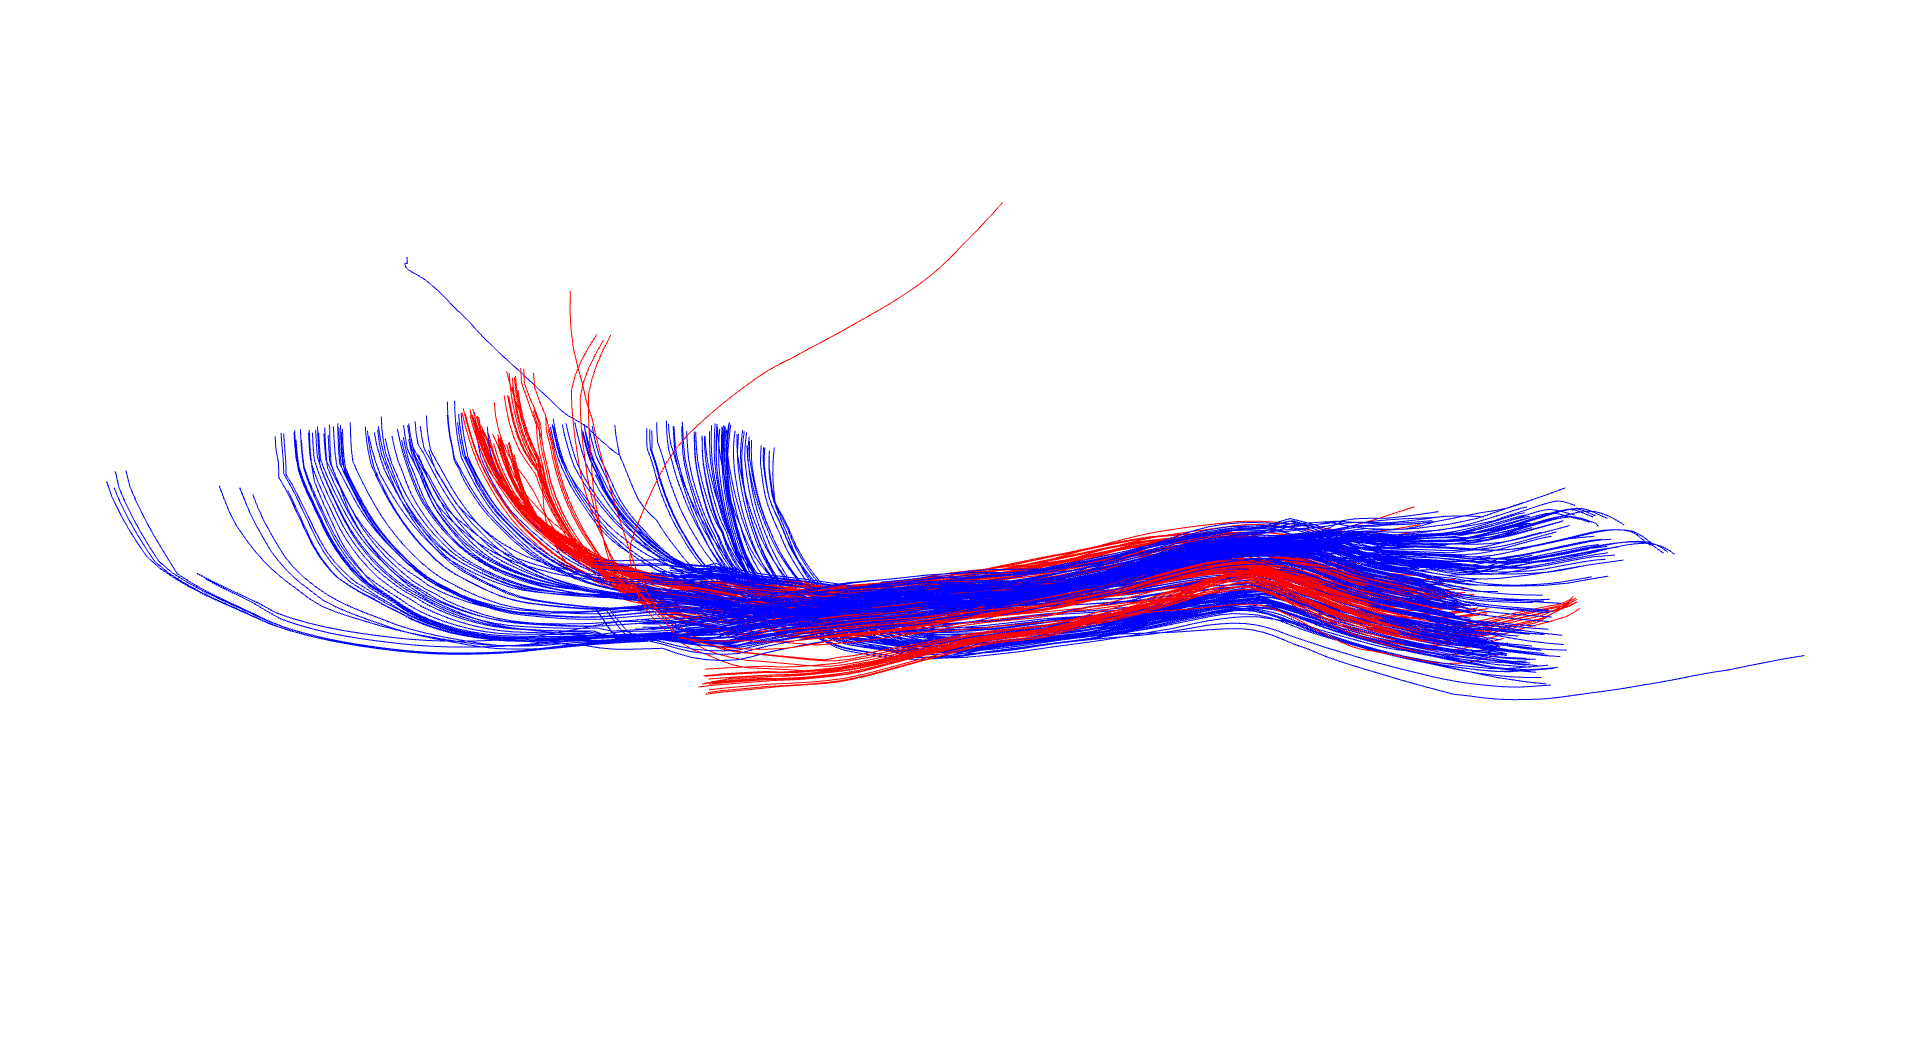
\includegraphics[scale=.3]{101_img_PCA}
\captionsetup{justification=centering}
\caption{The Orientation of ATR left side (red) as target bundle and right side of ATR (blue) as template bundle after applying PCA}
\label{fig:img_PCA}
\end{figure}

As we can see in the result of this experiment in Figure \ref{fig:img_PCA}, the PCA tool improved the alignment, so we go ahead and generate distances histogram as shown in Figure \ref{fig:hist_PCA} to select the threshold, which uses to build weights matrix. We also present the original distances histogram to show the improvement of the distances as well in Figure \ref{fig:hist_original}.

\begin{figure}[h!]
\centering
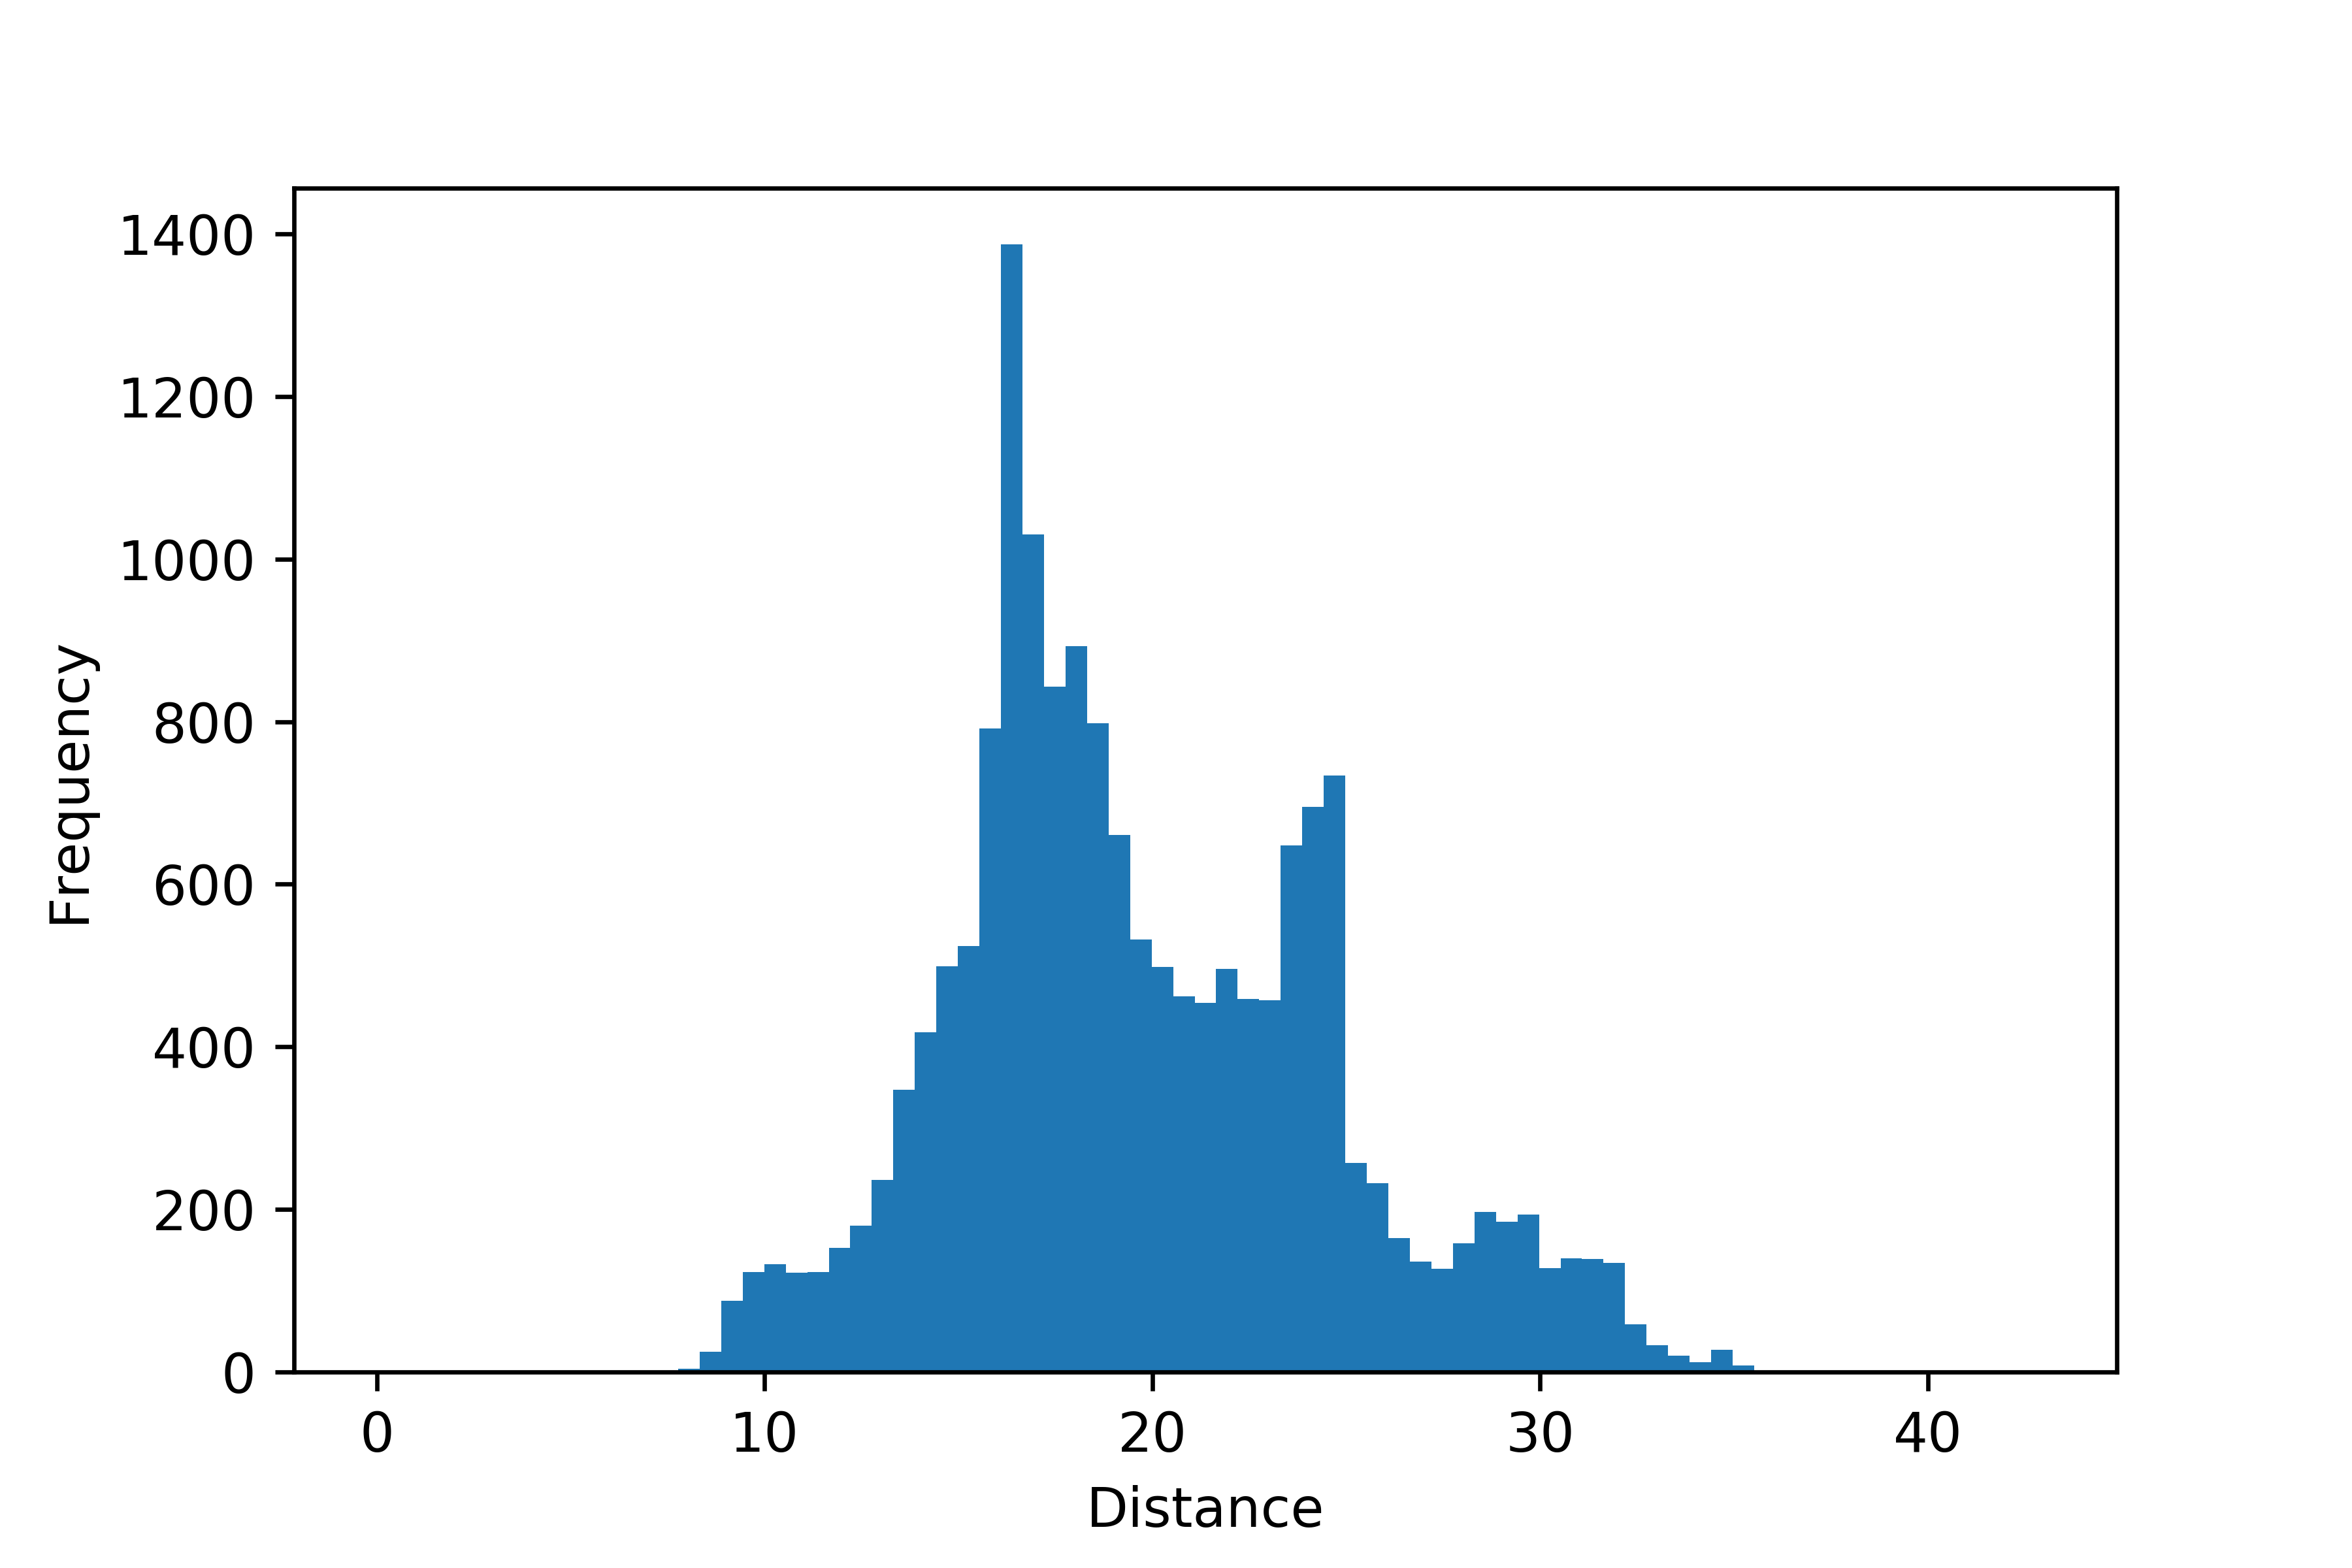
\includegraphics[scale=1]{110_hist_original}
\captionsetup{justification=centering}
\caption{The original distances histogram, it shows that the distances between points of template bundle and the points of target bundle lie between around thirty five and eight, and most of distances between fifteen and twenty five}
\label{fig:hist_original}
\end{figure}

\begin{figure}[h!]
\centering
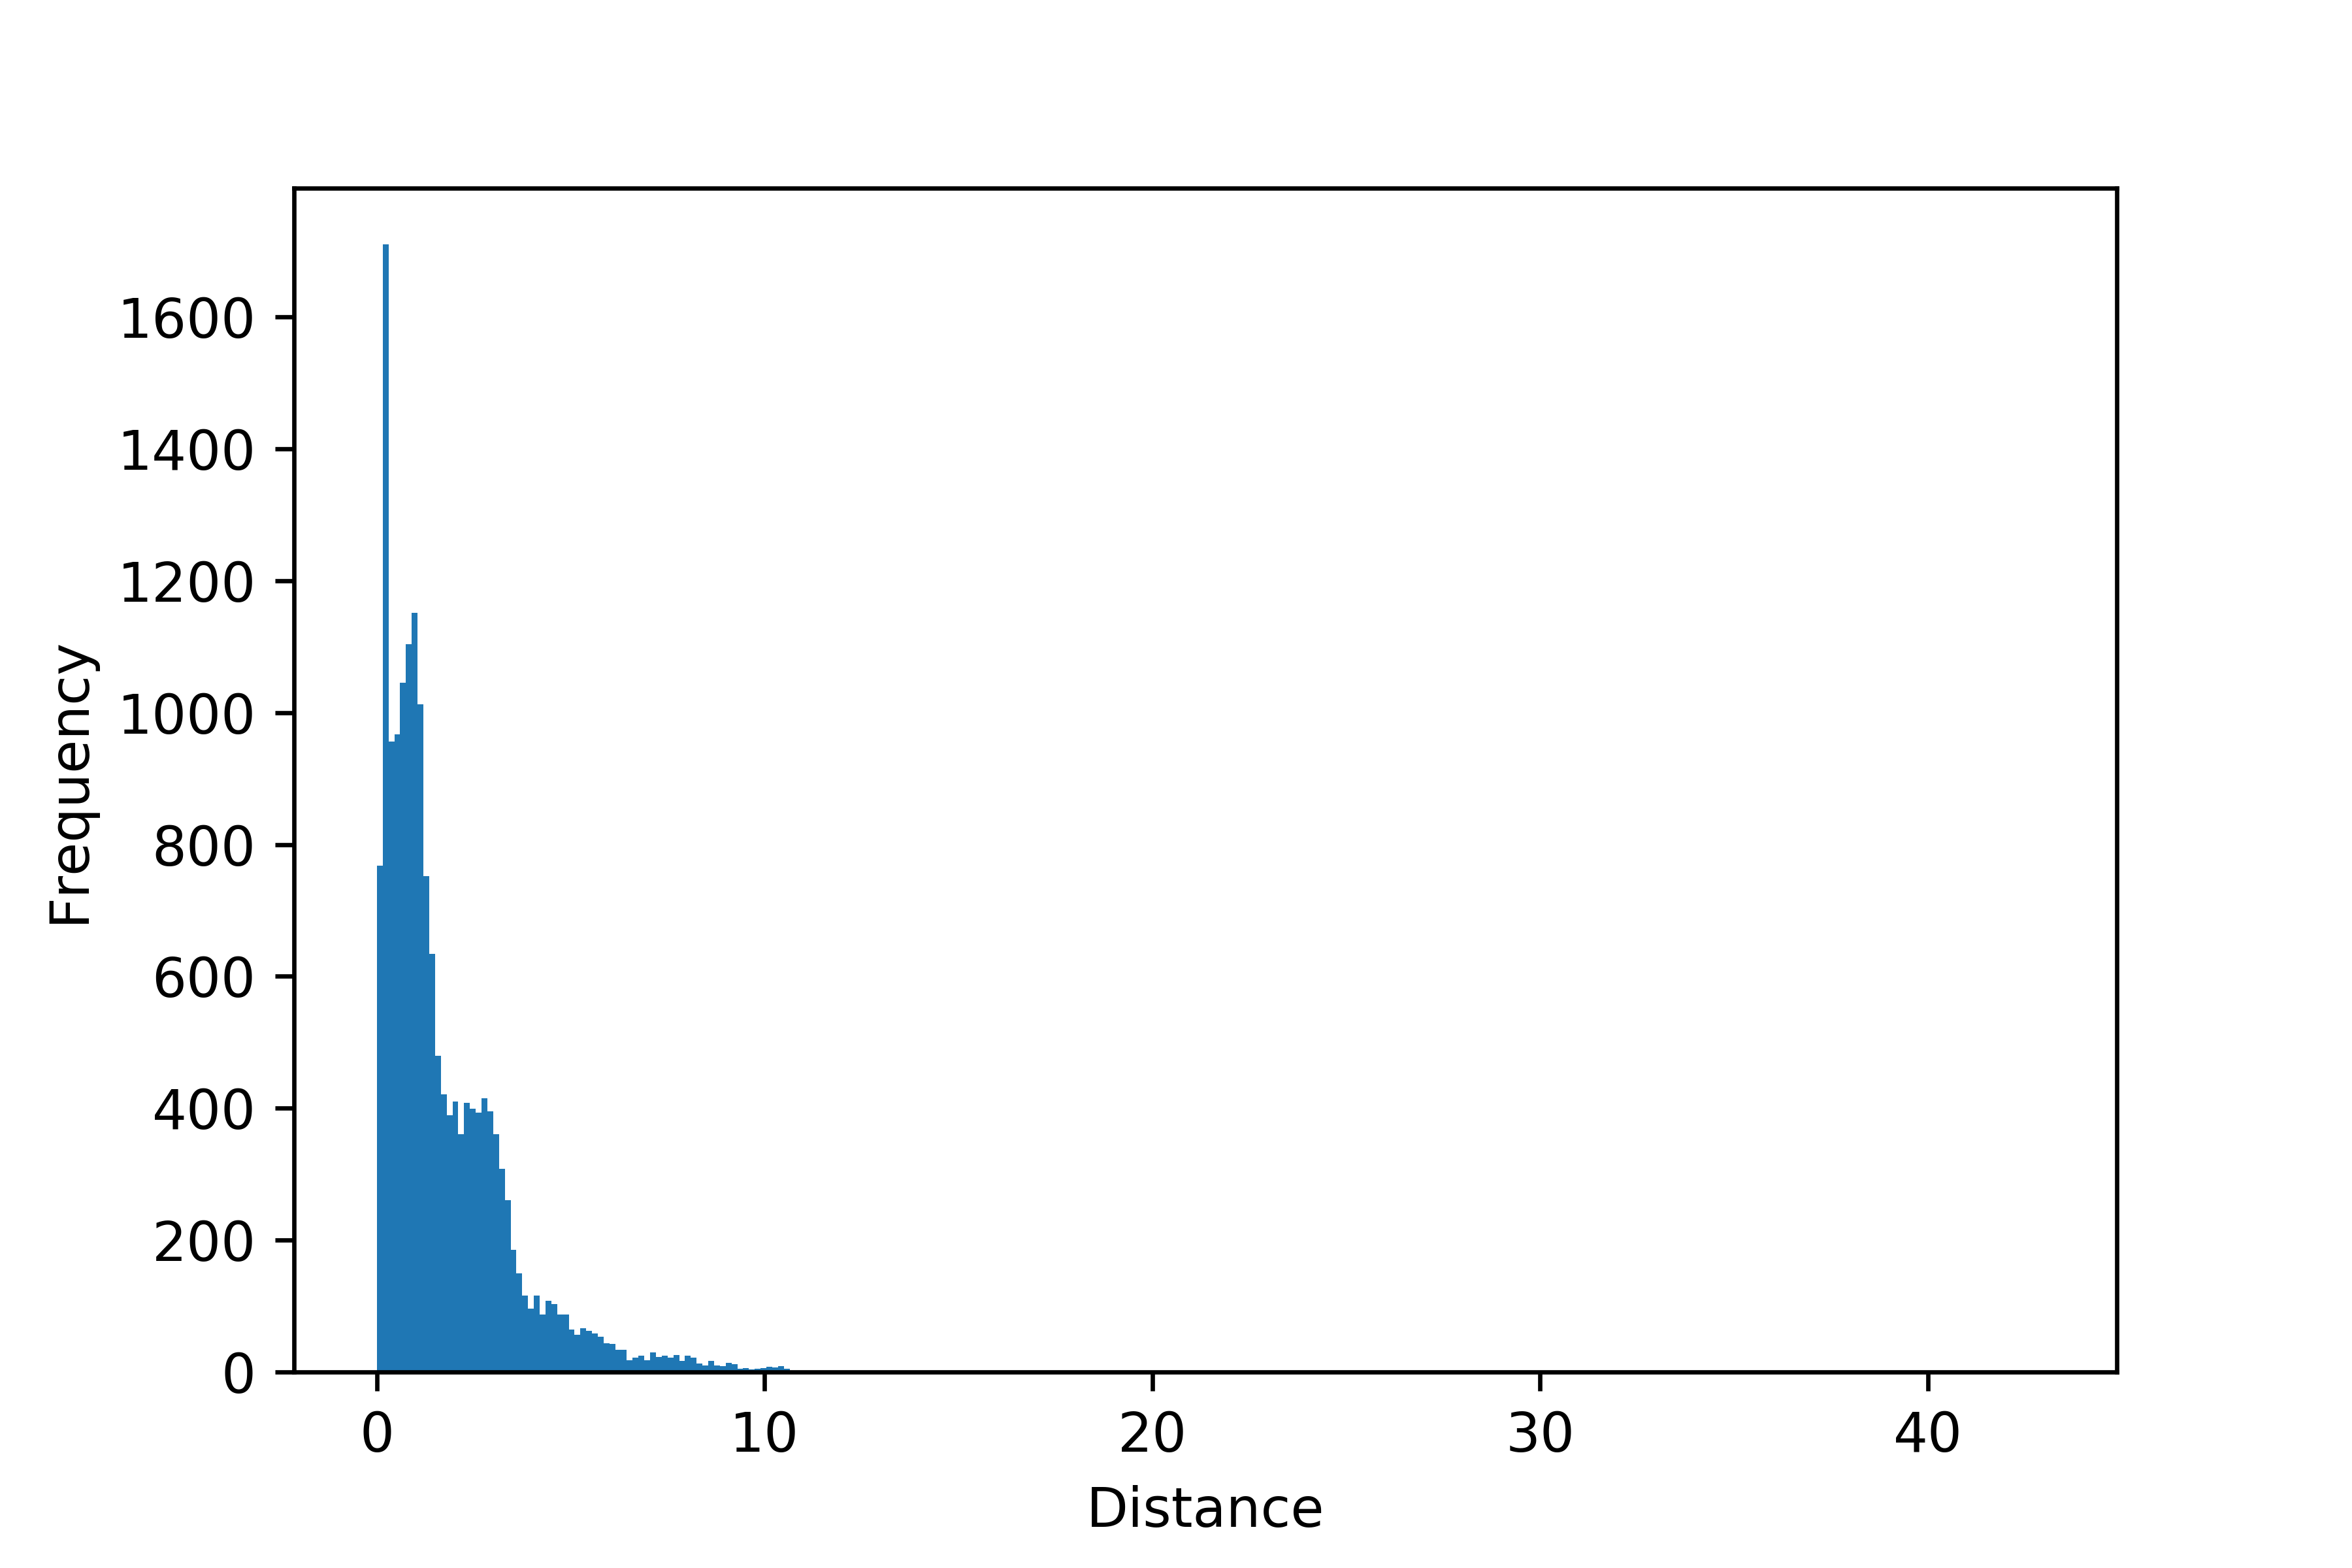
\includegraphics[scale=1]{110_hist_PCA}
\captionsetup{justification=centering}
\caption{Histogram of distances between template bundle and target bundle after applying PCA, it shows how PCA reduces the distances. Most of distances lie between zero and five}
\label{fig:hist_PCA}
\end{figure}

From the distances histogram in Figure \ref{fig:hist_PCA} we can choose the threshold to be seven, in that case, around ninety eight percent 98\% of points will have weight equal \textit{one} in the weight matrix $W$ and the remaining will be \textit{zero}.
\pagebreak

Now we need to select the stiffness weight $\alpha$, which is not trivial, it comes after observing the visual out of the registration. If the template bundle strongly deformed and it is about to map to target bundle, then we increase the value of $\alpha$ and vice versa. In this experiment we decide the optimal value of $\alpha$ is 999999.

The visual result of the registration is shown in Figure \ref{fig:hist_ICP}.
% we must put the results together
\begin{figure}[h!]
\centering
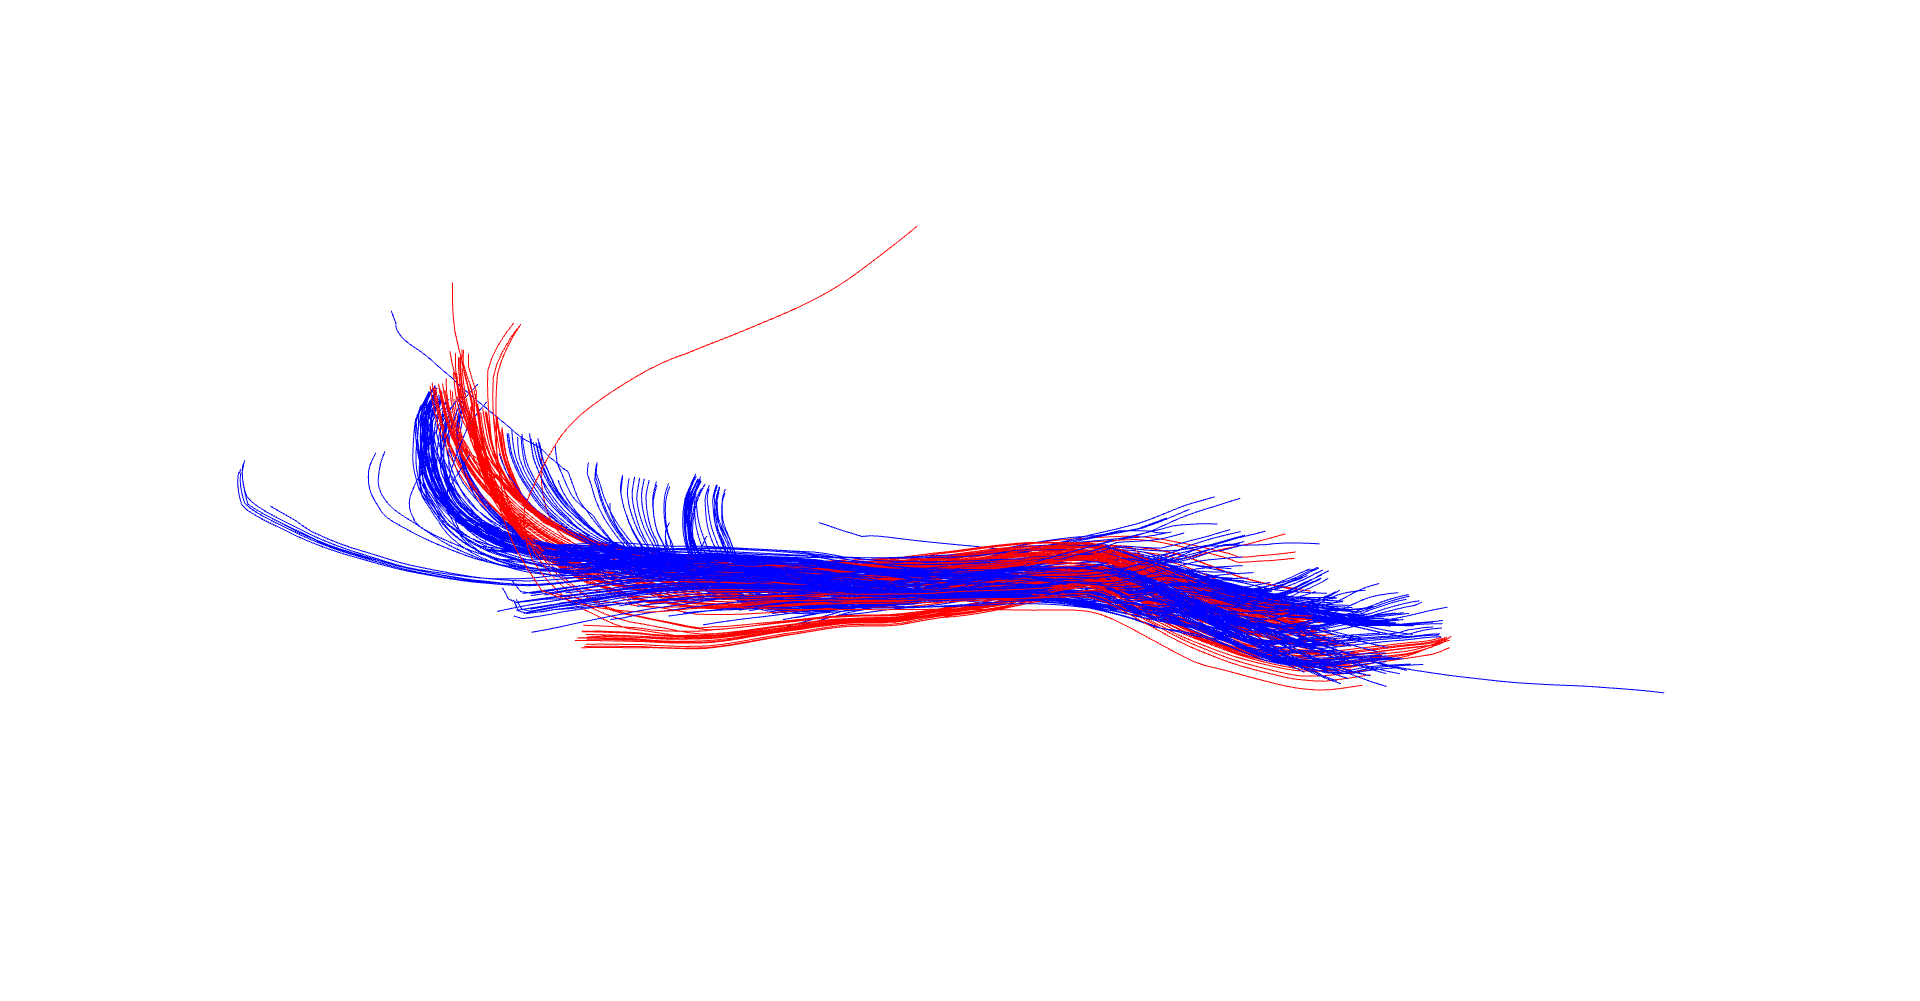
\includegraphics[scale=.4]{101_img_ICP}
\captionsetup{justification=centering}
\caption{The Orientation after ICP}
\label{fig:img_ICP}
\end{figure}

We also generate a histogram of distances to inspect the alignment improvement as shown in Figure \ref{fig:hist_ICP}

\begin{figure}[h!]
\centering
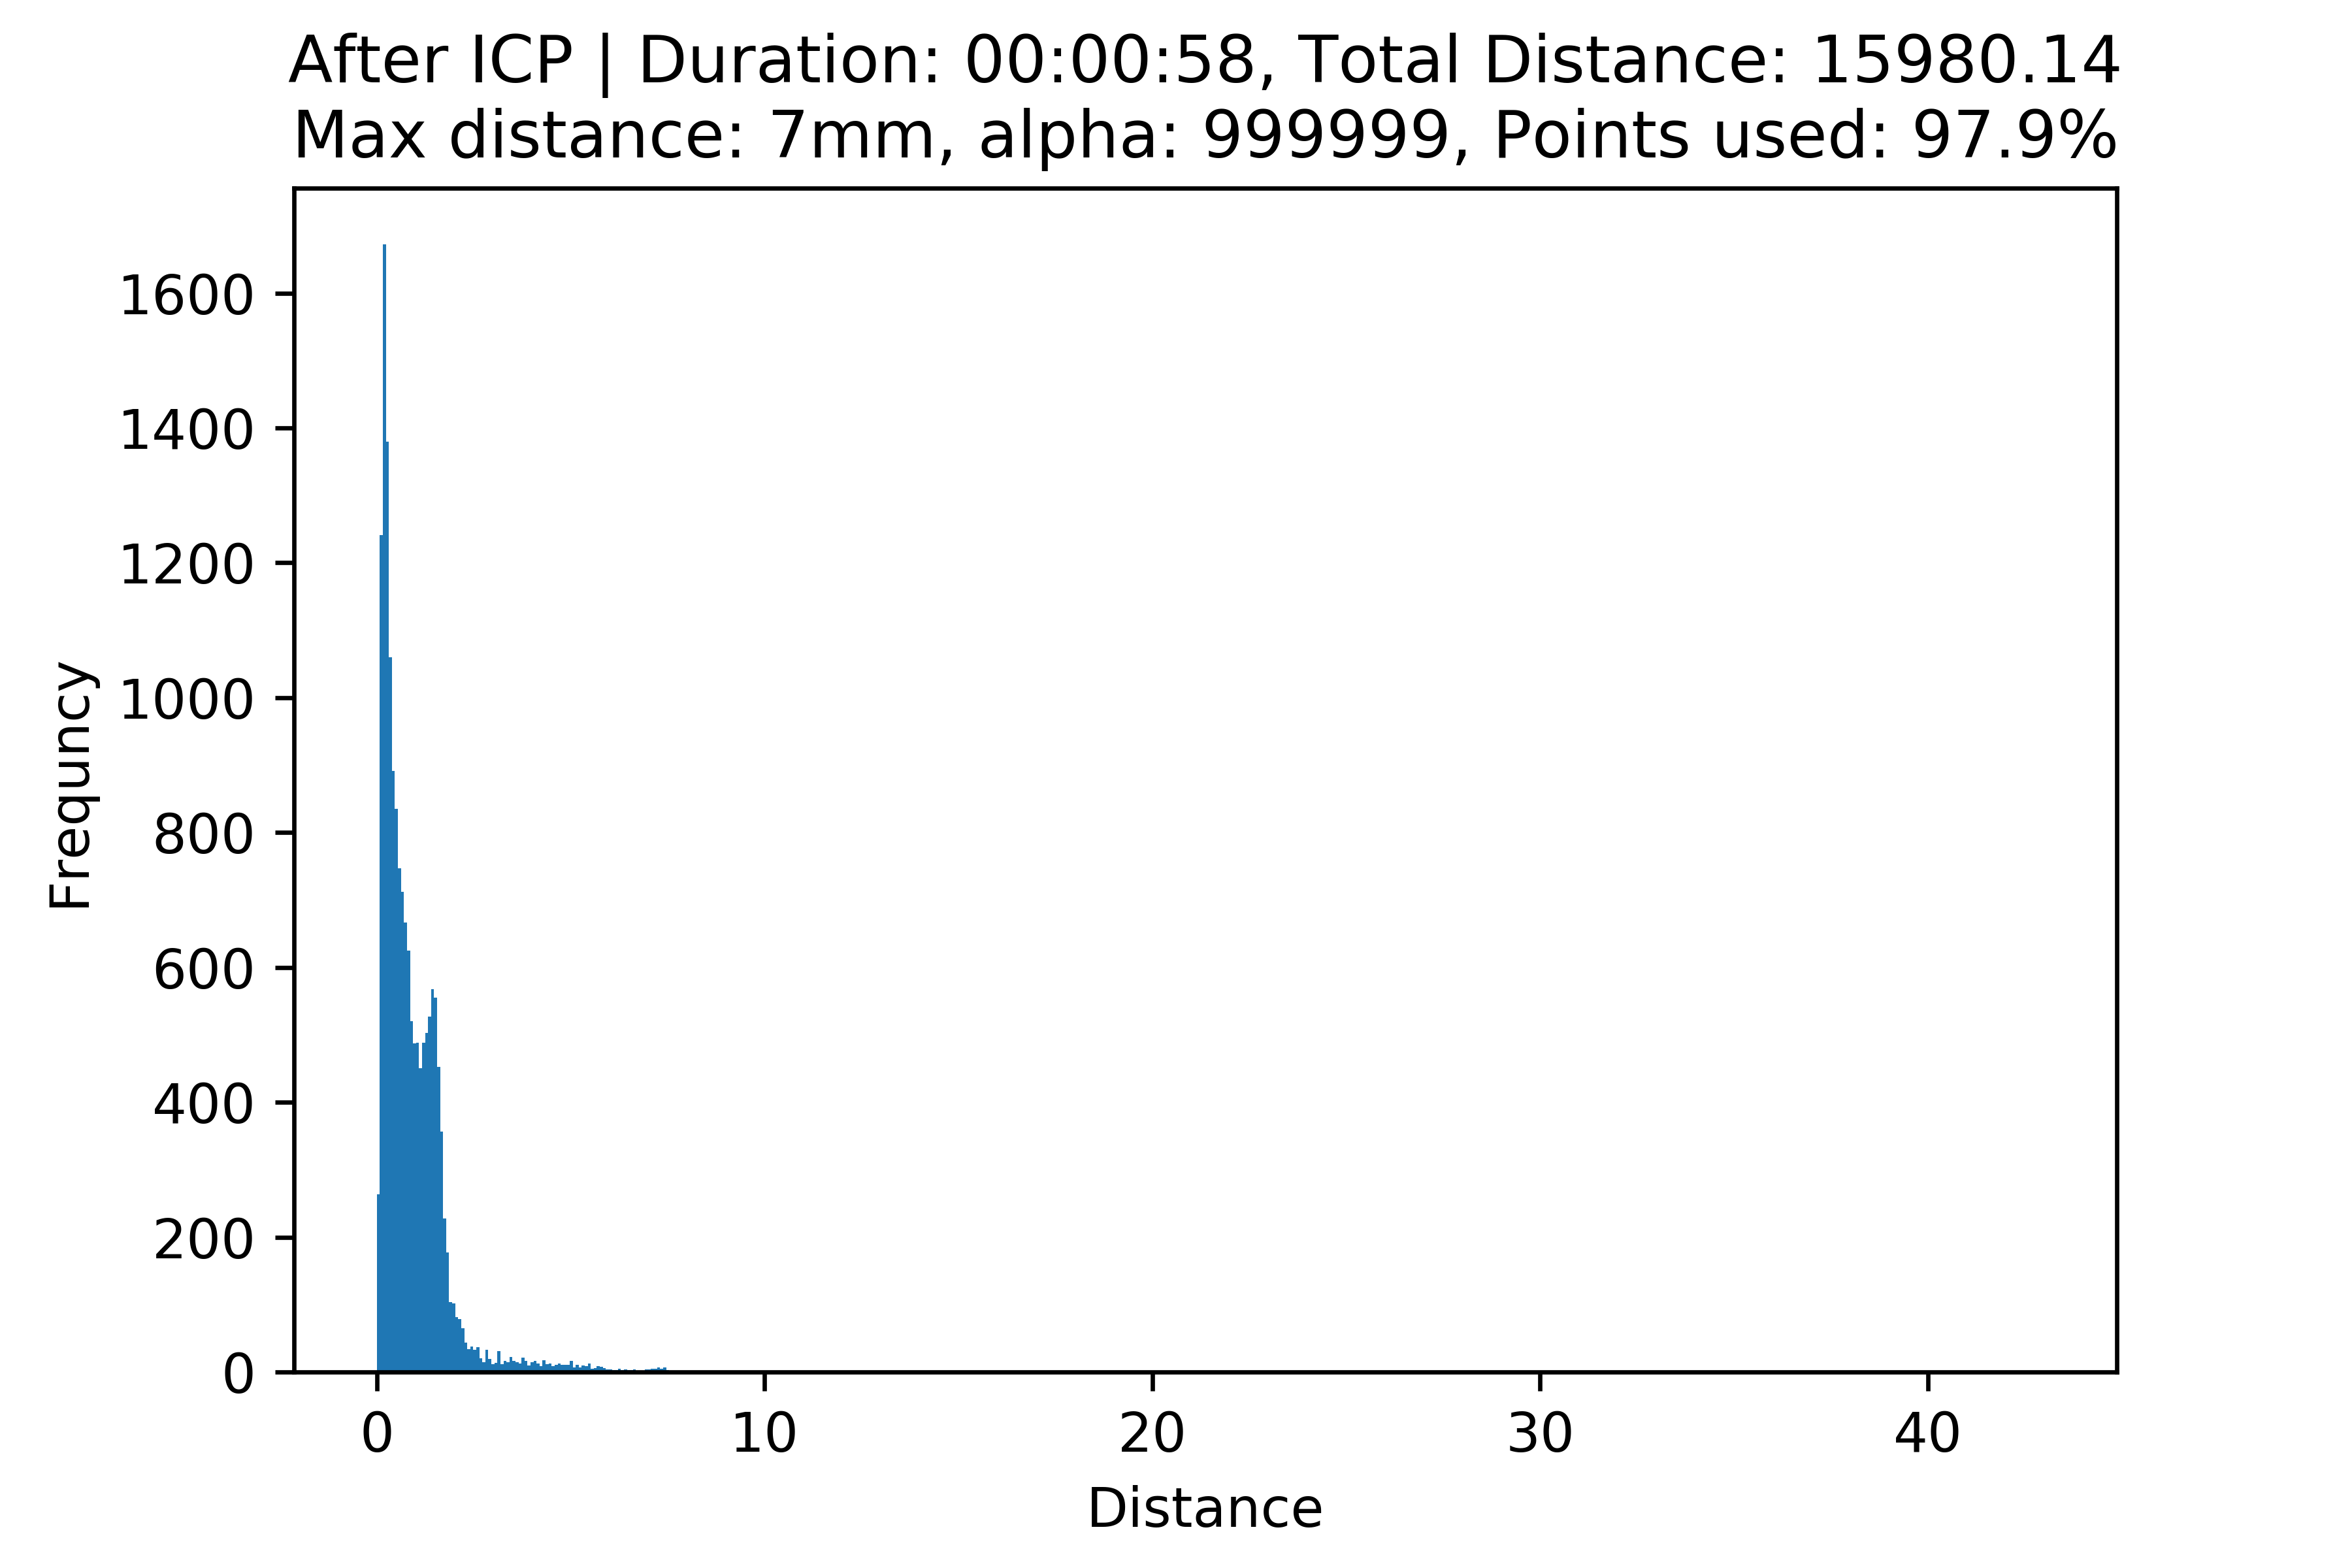
\includegraphics[scale=1]{101_hist_ICP}
\captionsetup{justification=centering}
\caption{The distances histogram after ICP}
\label{fig:hist_ICP}
\end{figure}

We register the same bundles with \textit{DIPY} method to compare it with our method. As we mention before, we use the bundles after PCA alignment here as well because DIPY fails to have sufficient initial alignment between pathways in different sides of the brain, but it can accepting an affine matrix as parameter as initial orientation. To solve this problem, we use the PCA tool that we develop to initiate the position of template bundle. The visual result of DIPY registration is shown in Figures \ref{fig:img_dipy} and we put again here the visual result of our tool ease the comparison.

\begin{figure}[h!]
\centering
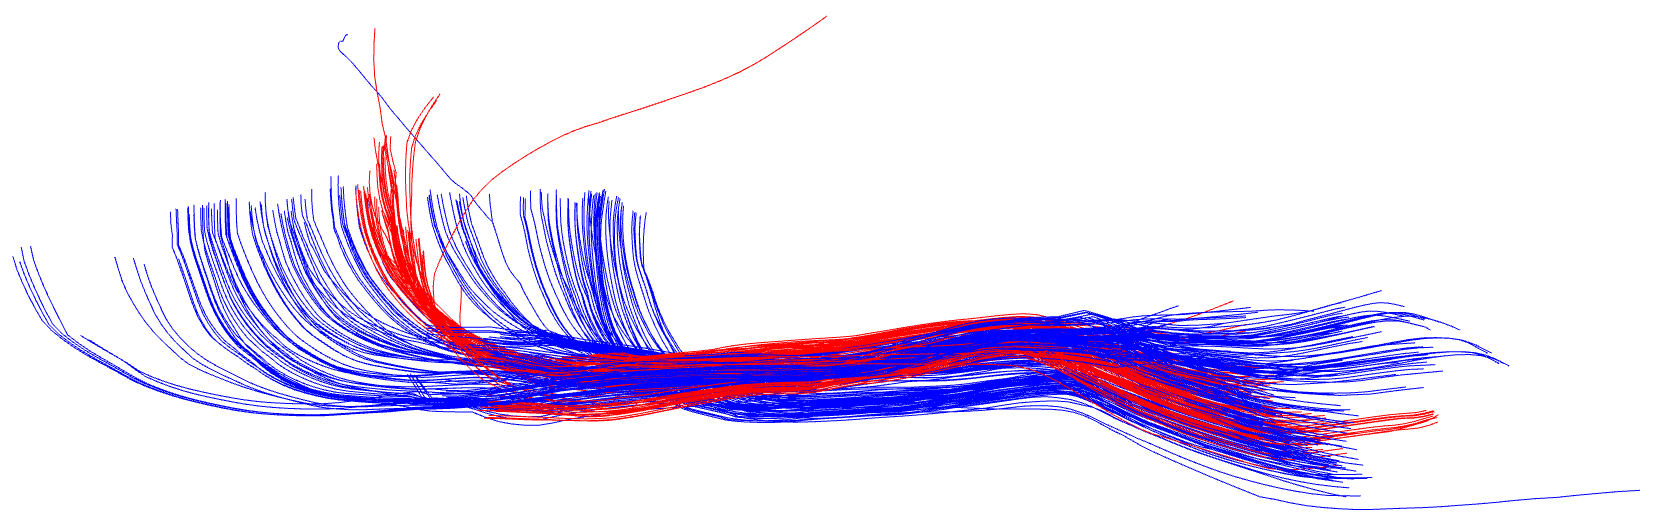
\includegraphics[scale=.3]{101_img_dipy}
\captionsetup{justification=centering}
\caption{The Orientation after DIPY}
\label{fig:img_dipy}
\end{figure}

\begin{figure}[h!]
\centering
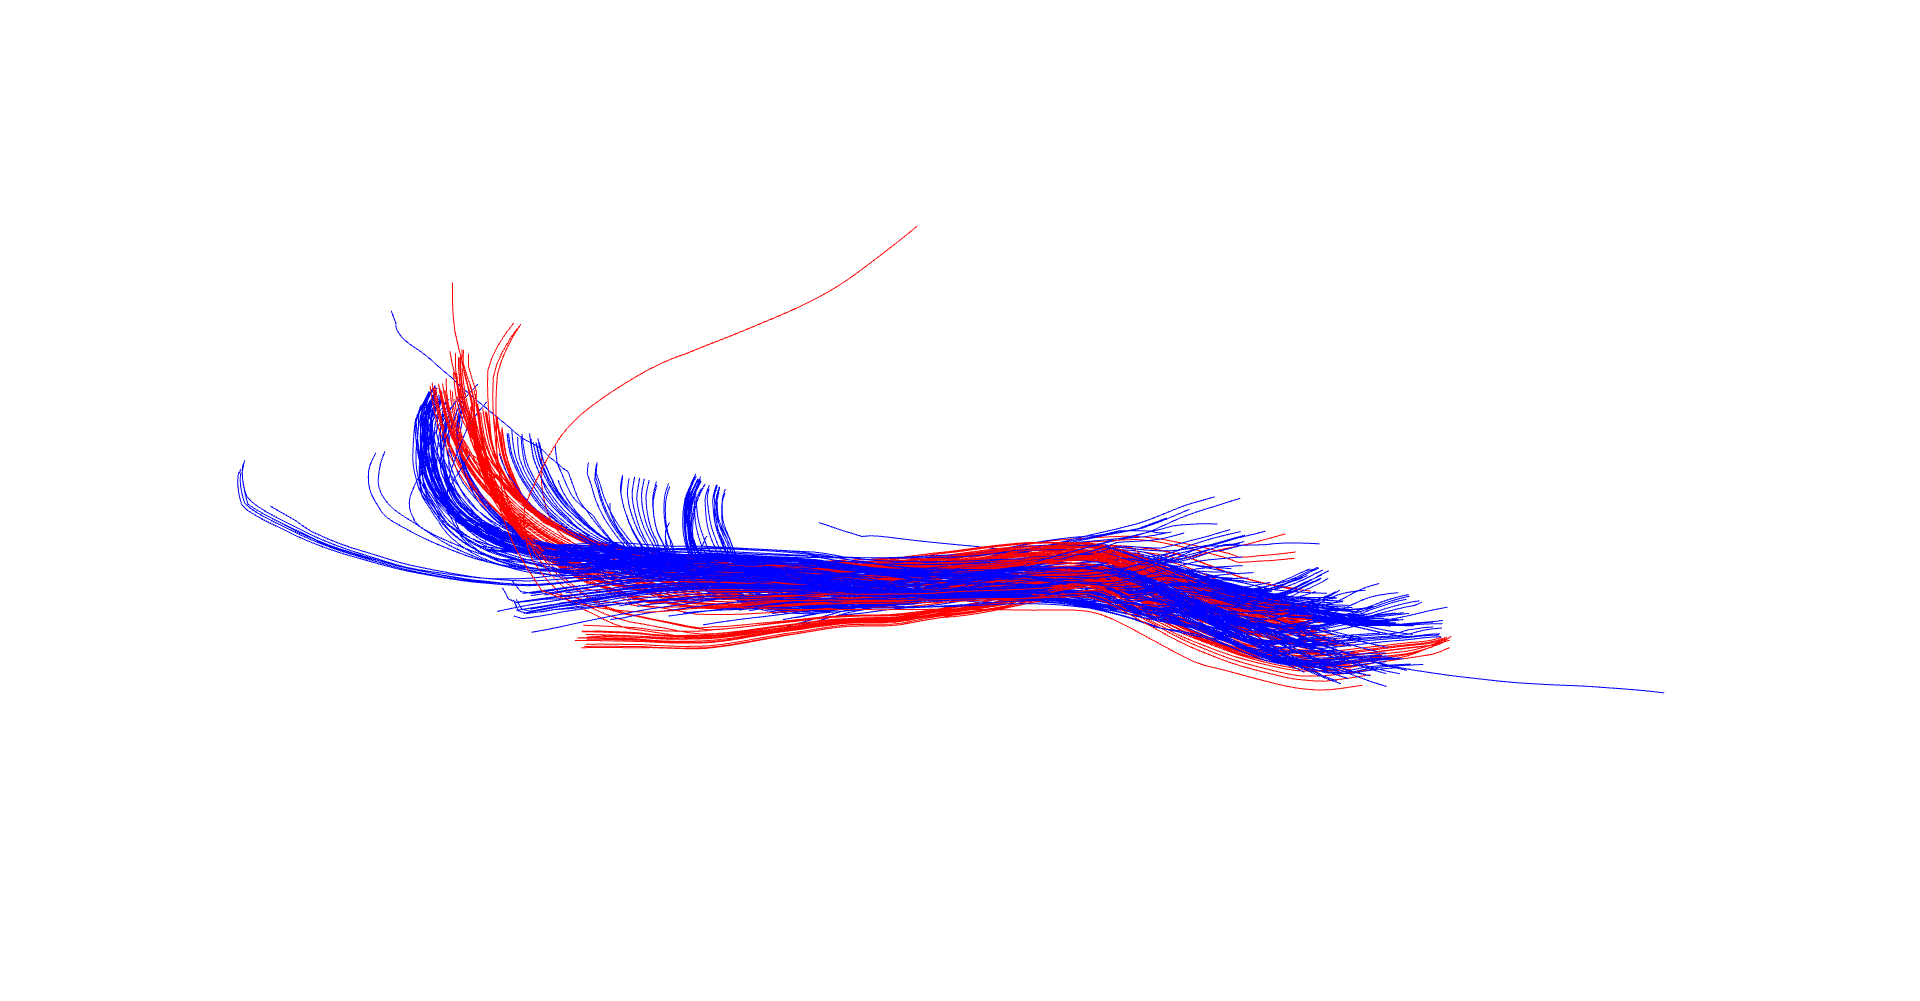
\includegraphics[scale=.4]{101_img_ICP}
\captionsetup{justification=centering}
\caption{The Orientation after ICP}
\label{fig:img_ICP}
\end{figure}

And we present the distances histograms after registration our tool and after registering using DIPY in Figures 

\begin{figure}[h!]
\centering
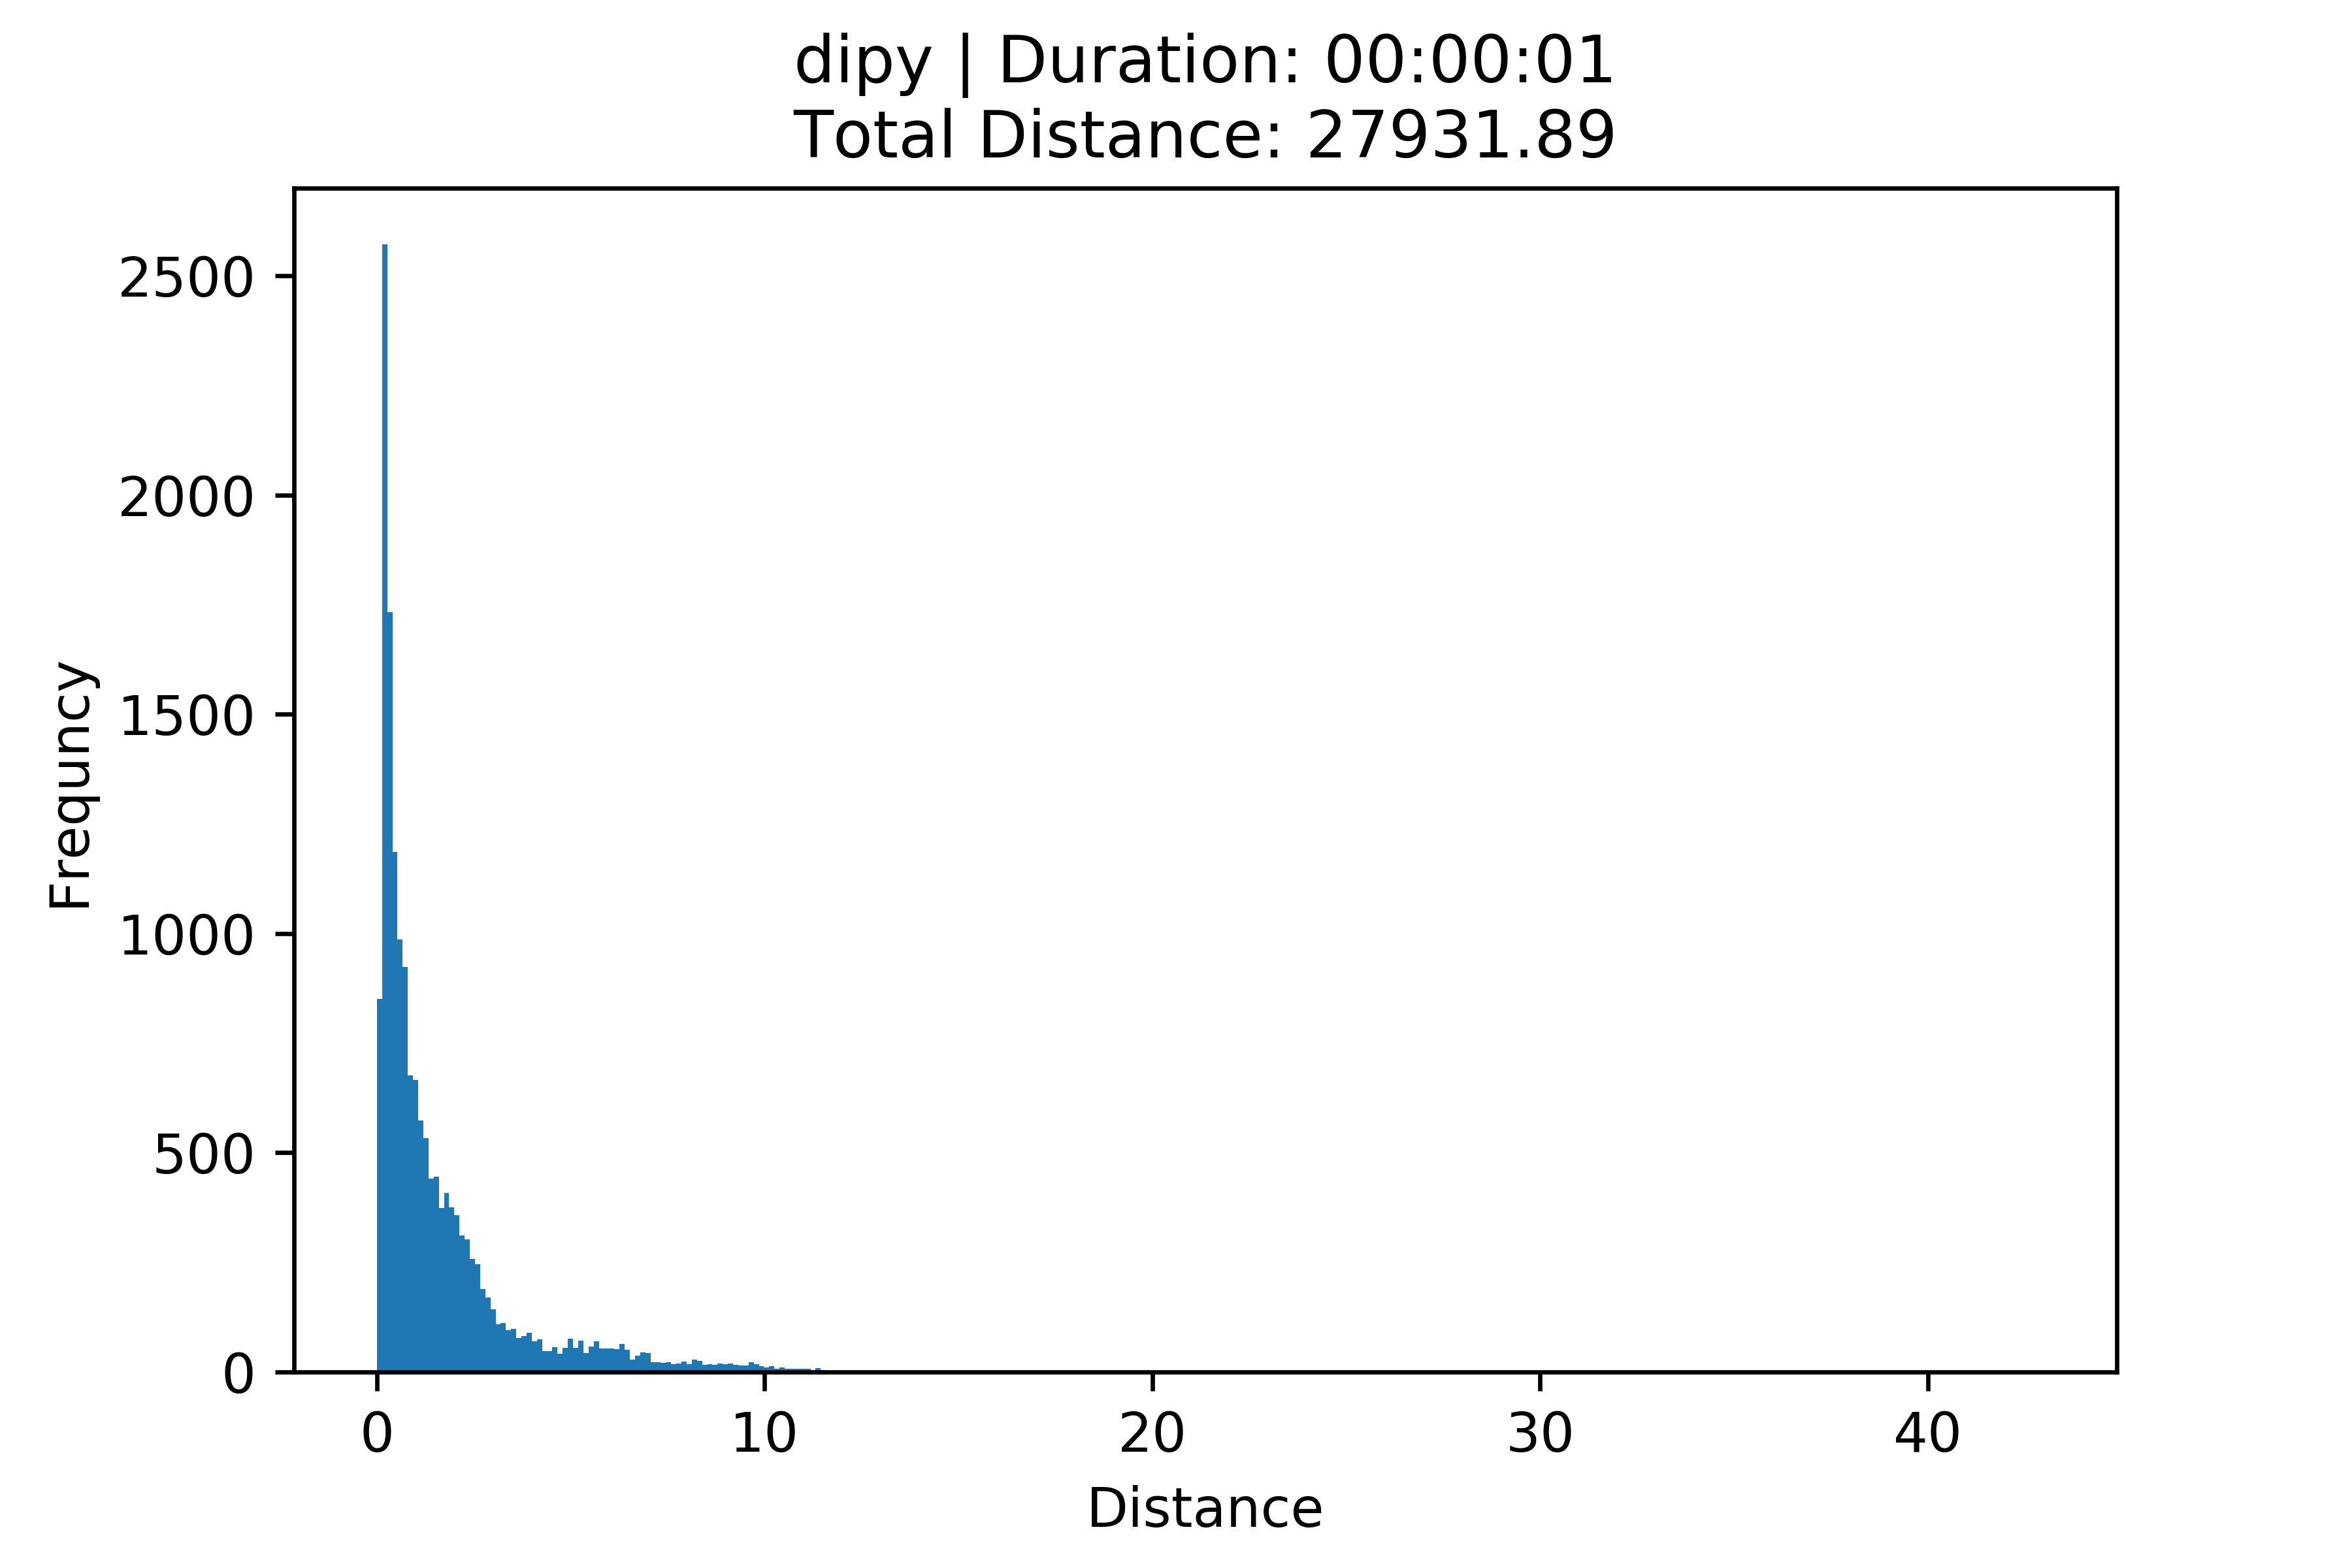
\includegraphics[scale=1]{101_dipy_hist}
\captionsetup{justification=centering}
\caption{The distances histogram after DIPY}
\label{fig:dipy_hist}
\end{figure}

\begin{figure}[h!]
\centering
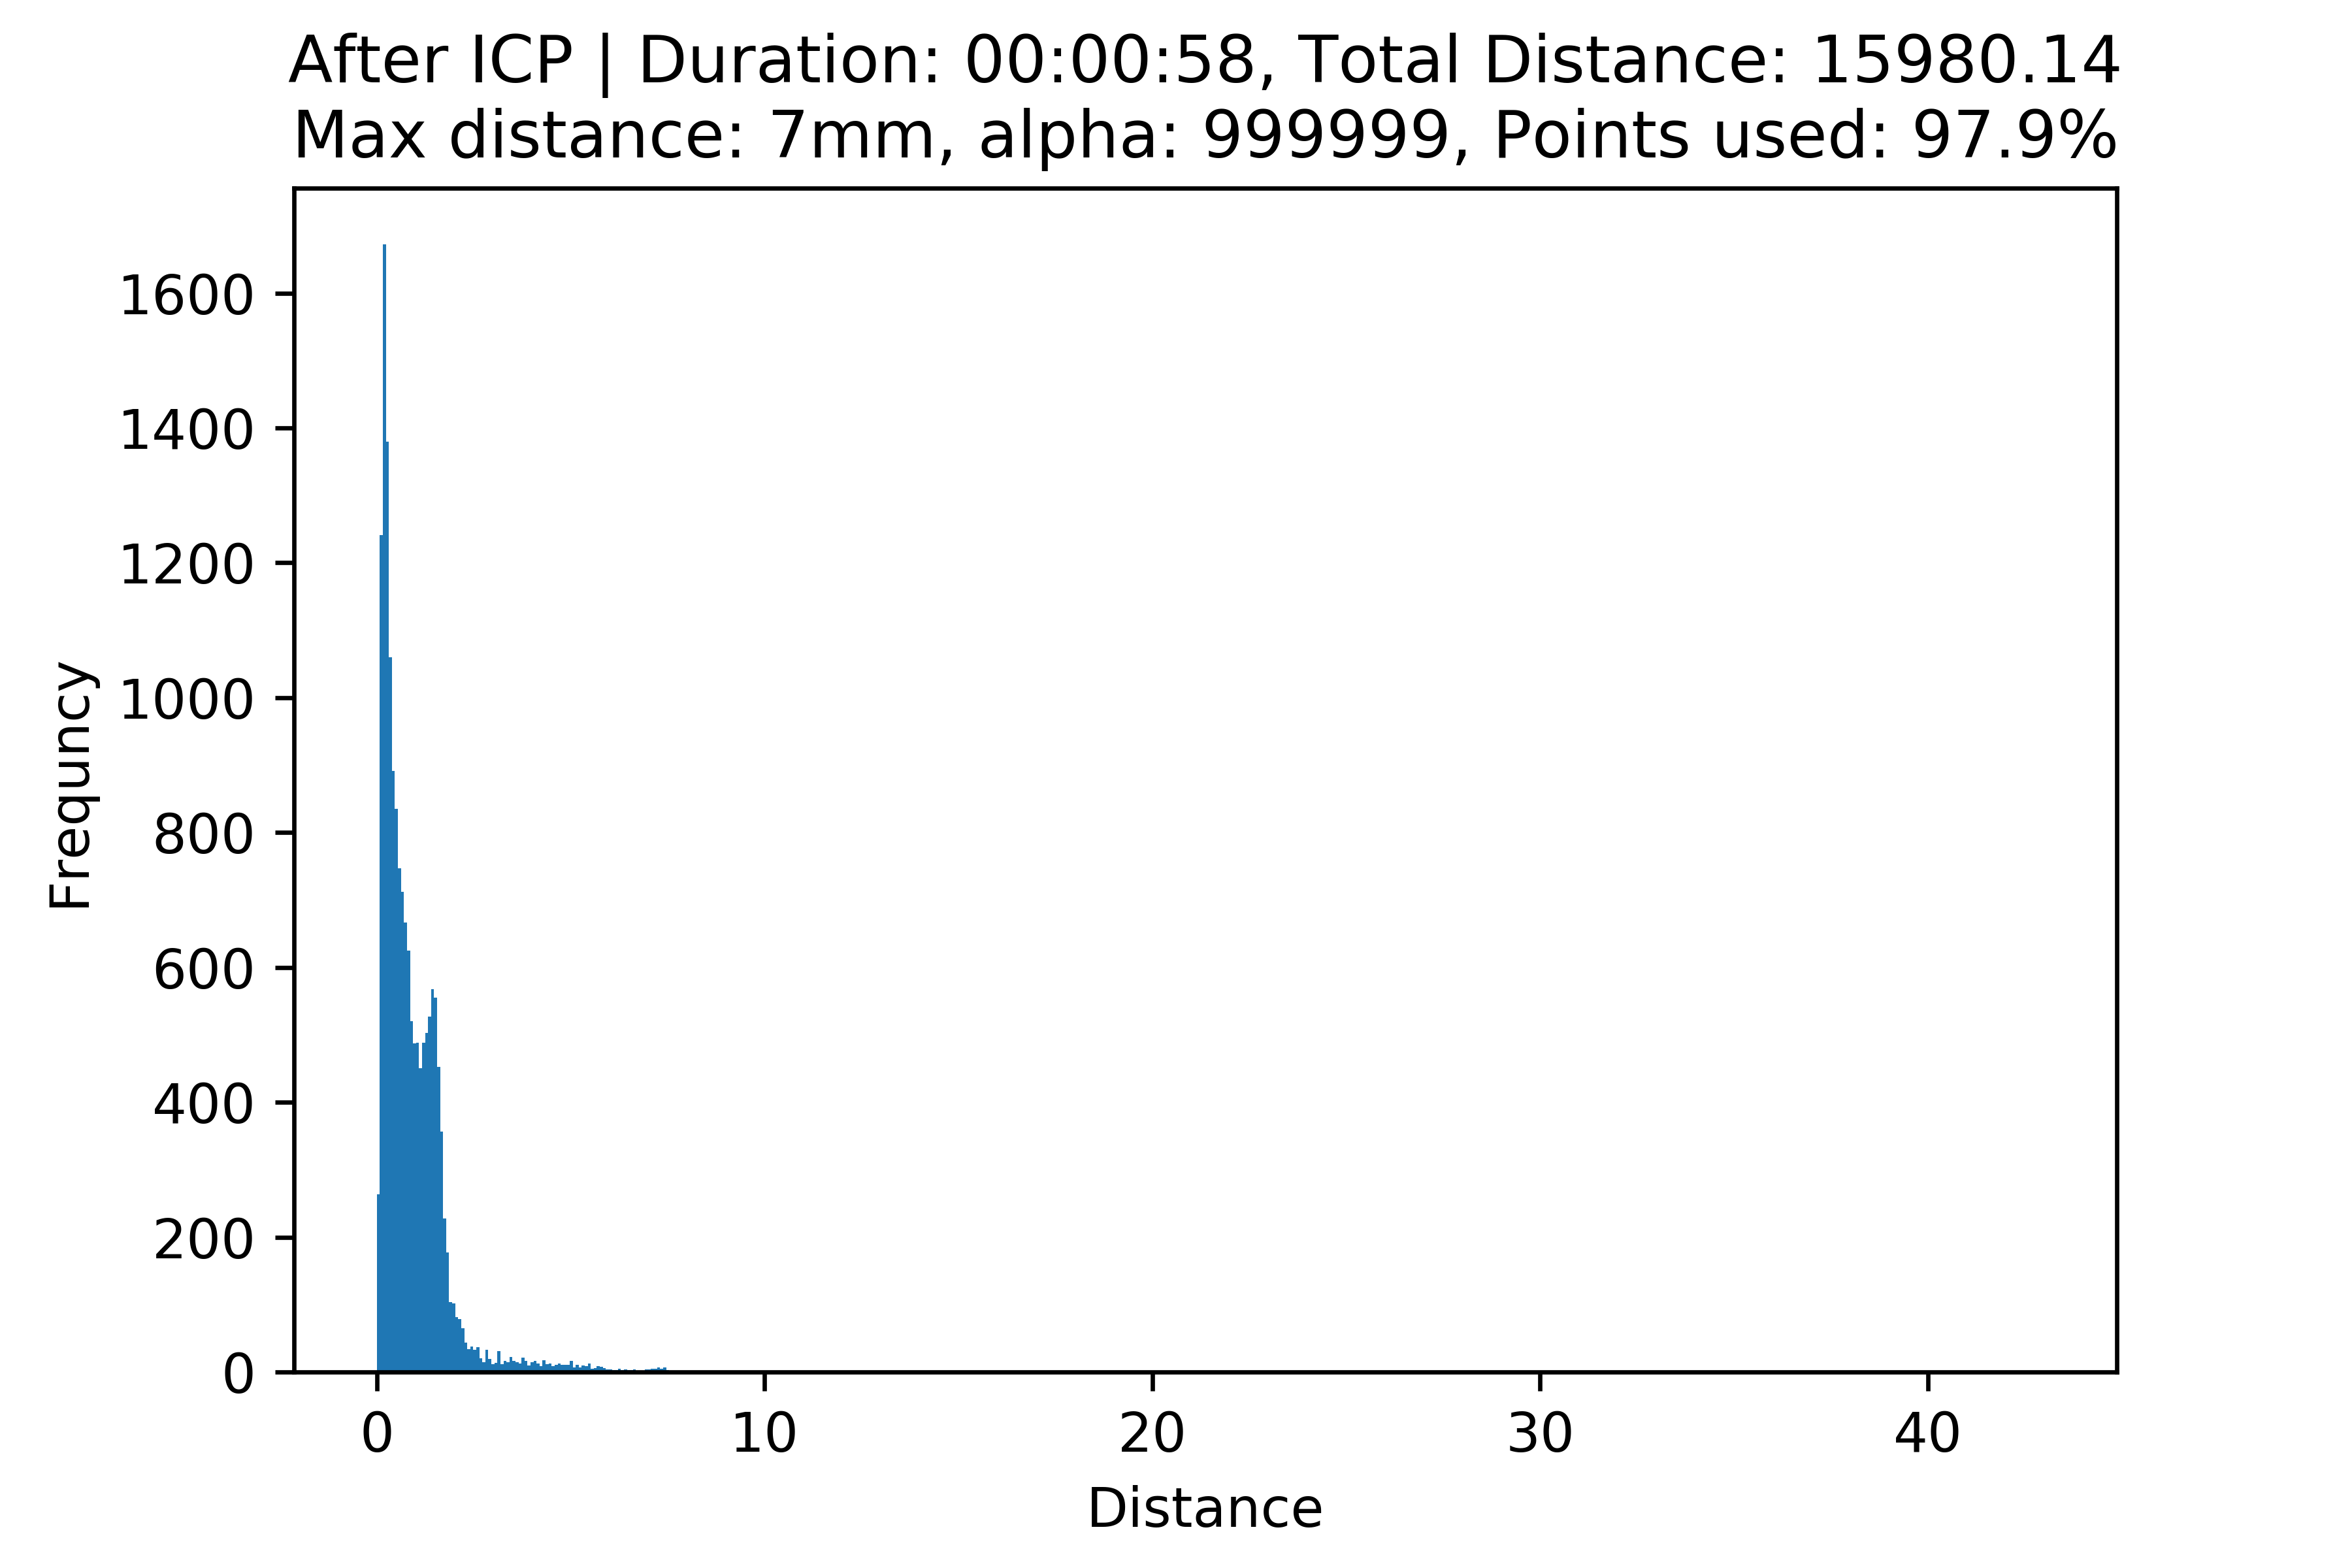
\includegraphics[scale=1]{101_hist_ICP}
\captionsetup{justification=centering}
\caption{The distances histogram after ICP}
\label{fig:hist_ICP}
\end{figure}

\section{Experiment (2)}
The second experiment is measuring how the method can correct the deformation. Therefore, we toke the right side of ATR and deform its shape, then we register it with the original copy before deformation. As we can see in Figures , the tool can correct the deformation appropriately.

\begin{figure}[h!]
\centering
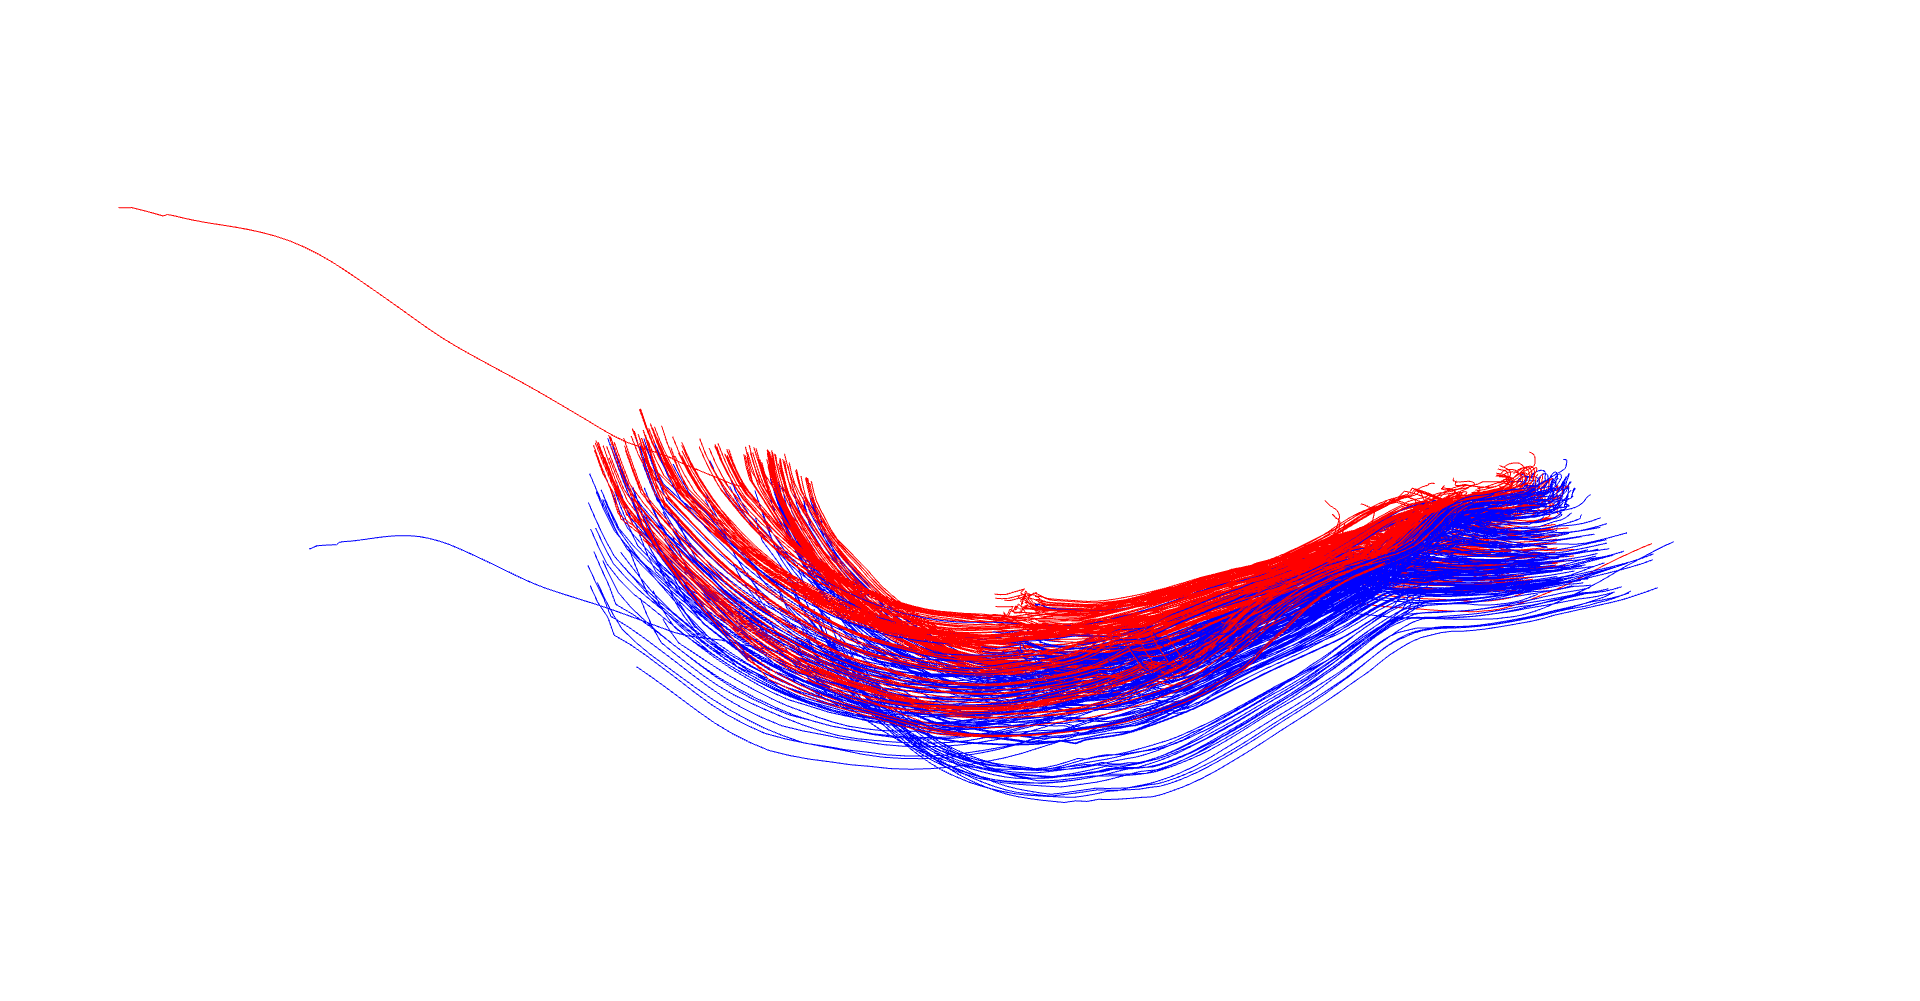
\includegraphics[scale=.3]{102_img_original}
\captionsetup{justification=centering}
\caption{The orientation after deformation}
\label{fig:img_original_def}
\end{figure}

Also, we put the distances histograms before and after registration in Figures 

\begin{figure}[h!]
\centering
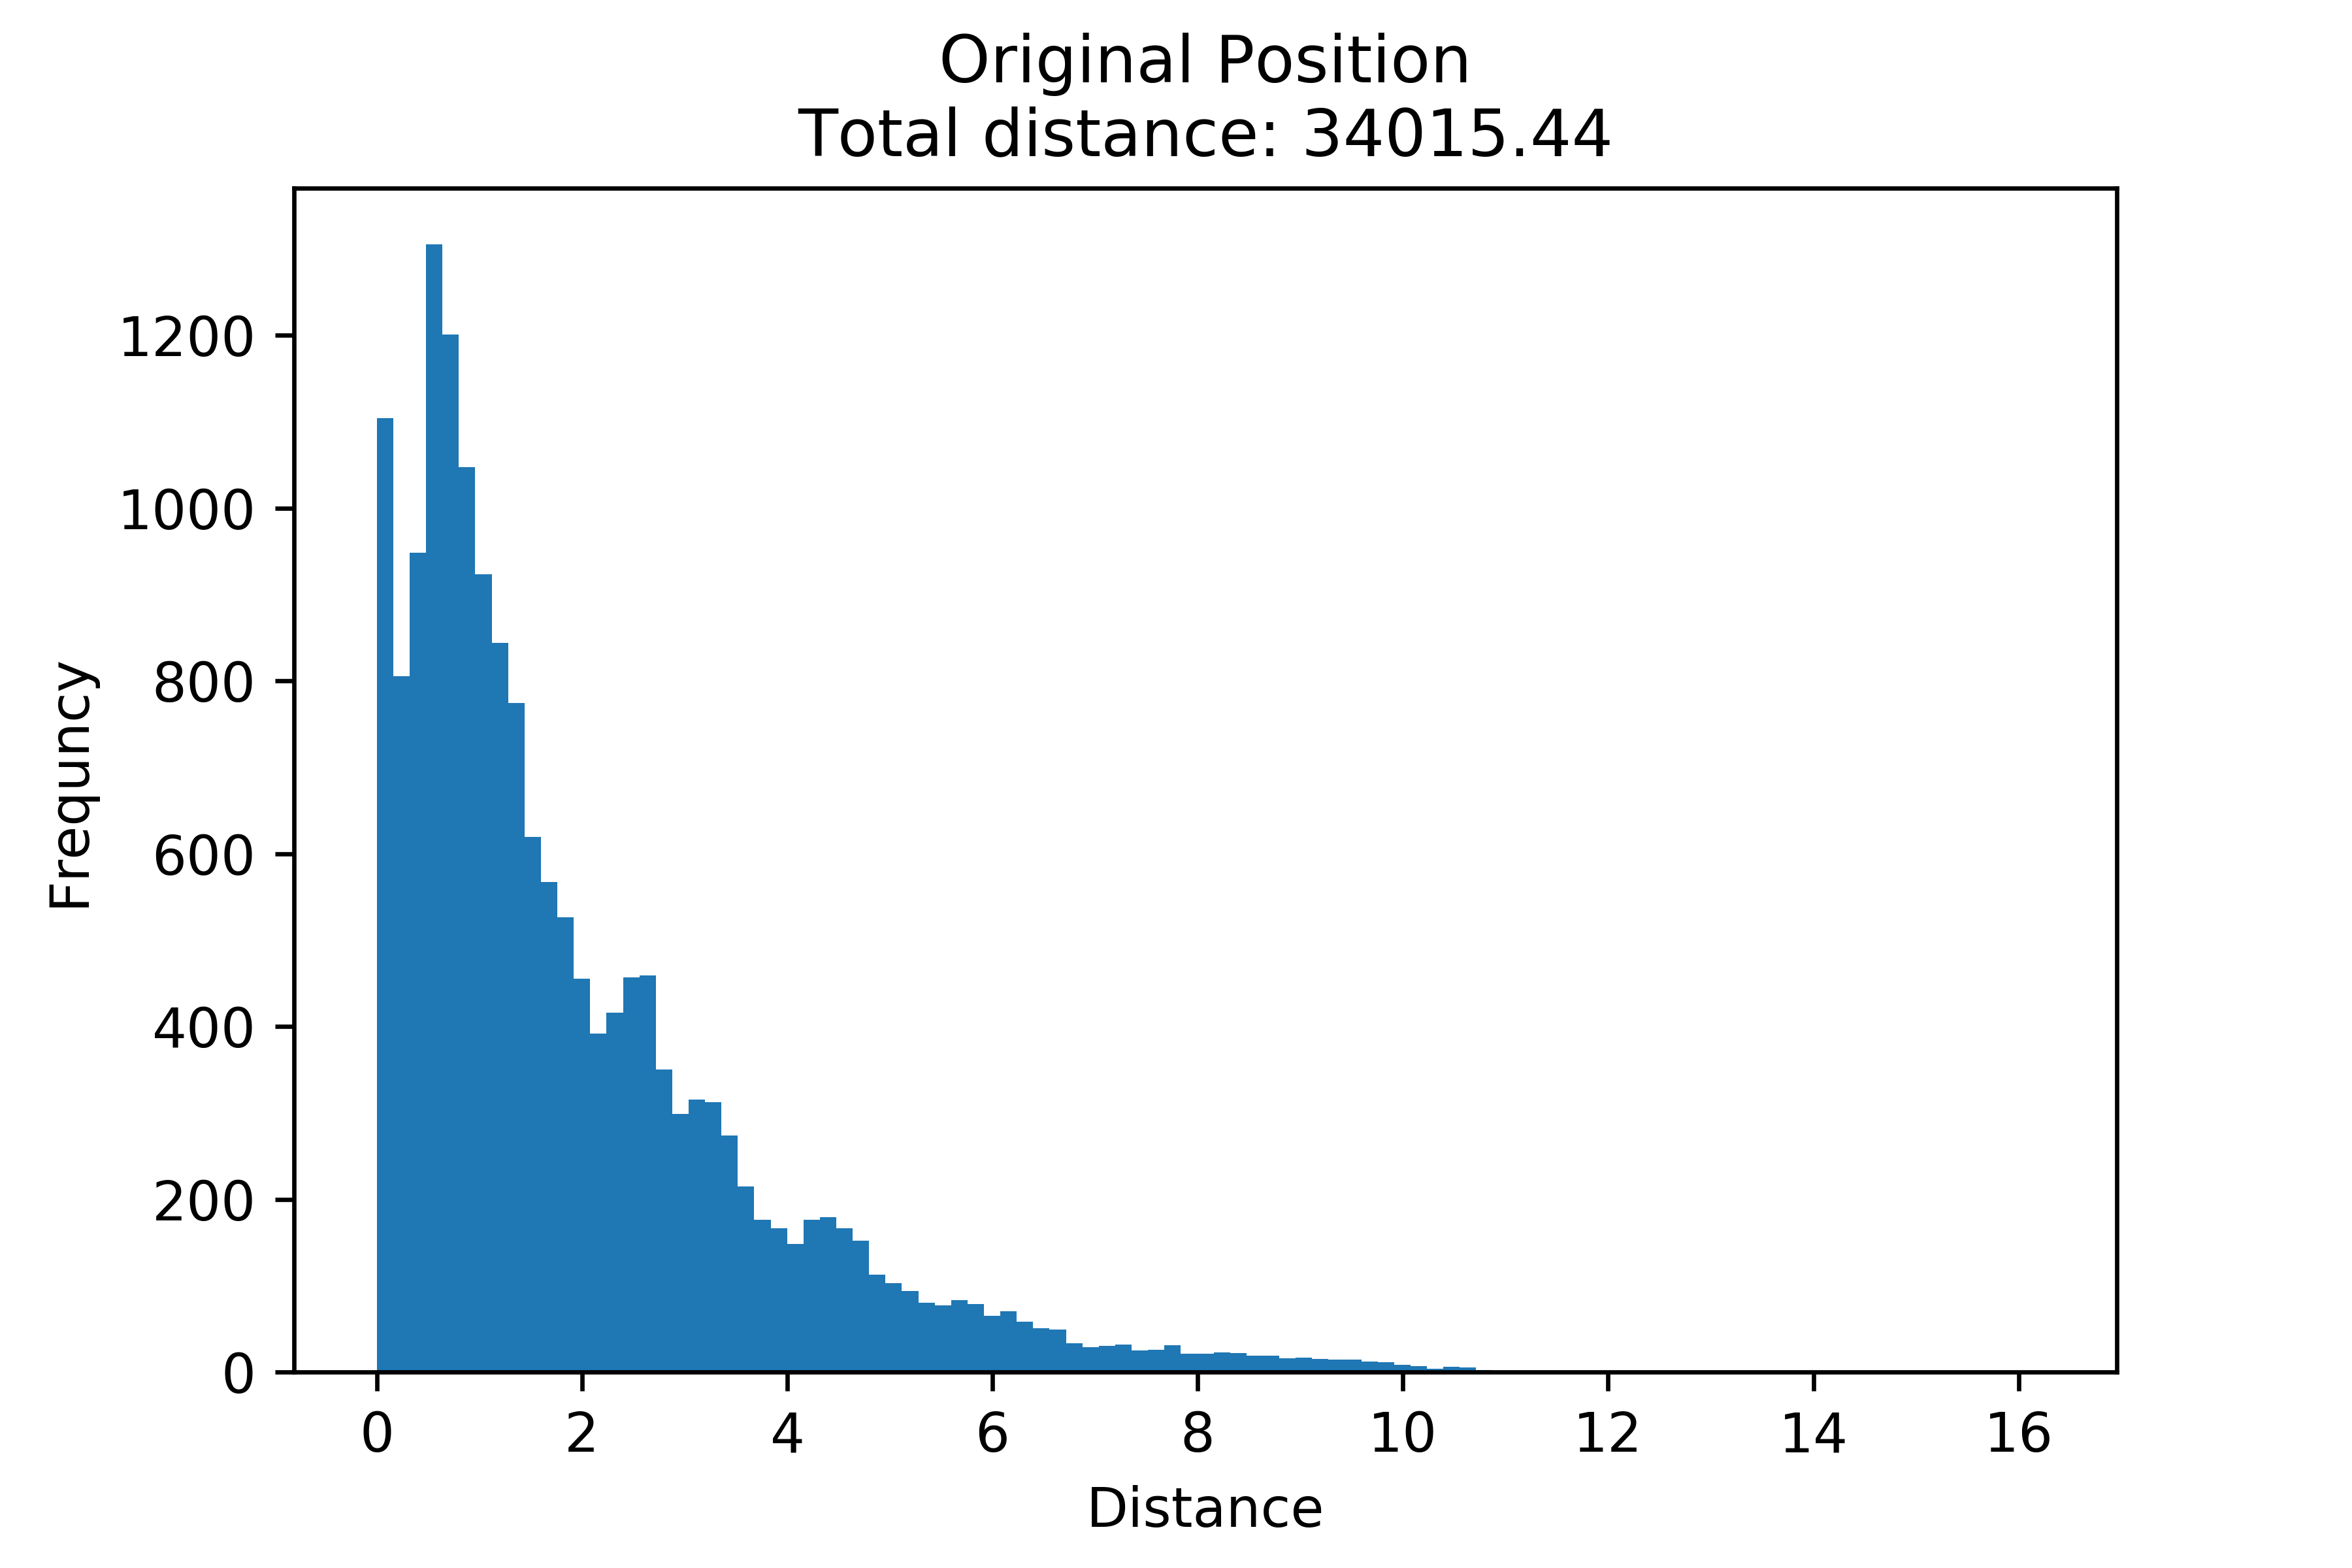
\includegraphics[scale=1]{102_hist_original}
\captionsetup{justification=centering}
\caption{The distances histogram after deforming a bundle and measuring the distances from the original one}
\label{fig:hist_original_def}
\end{figure}

\begin{figure}[h!]
\centering
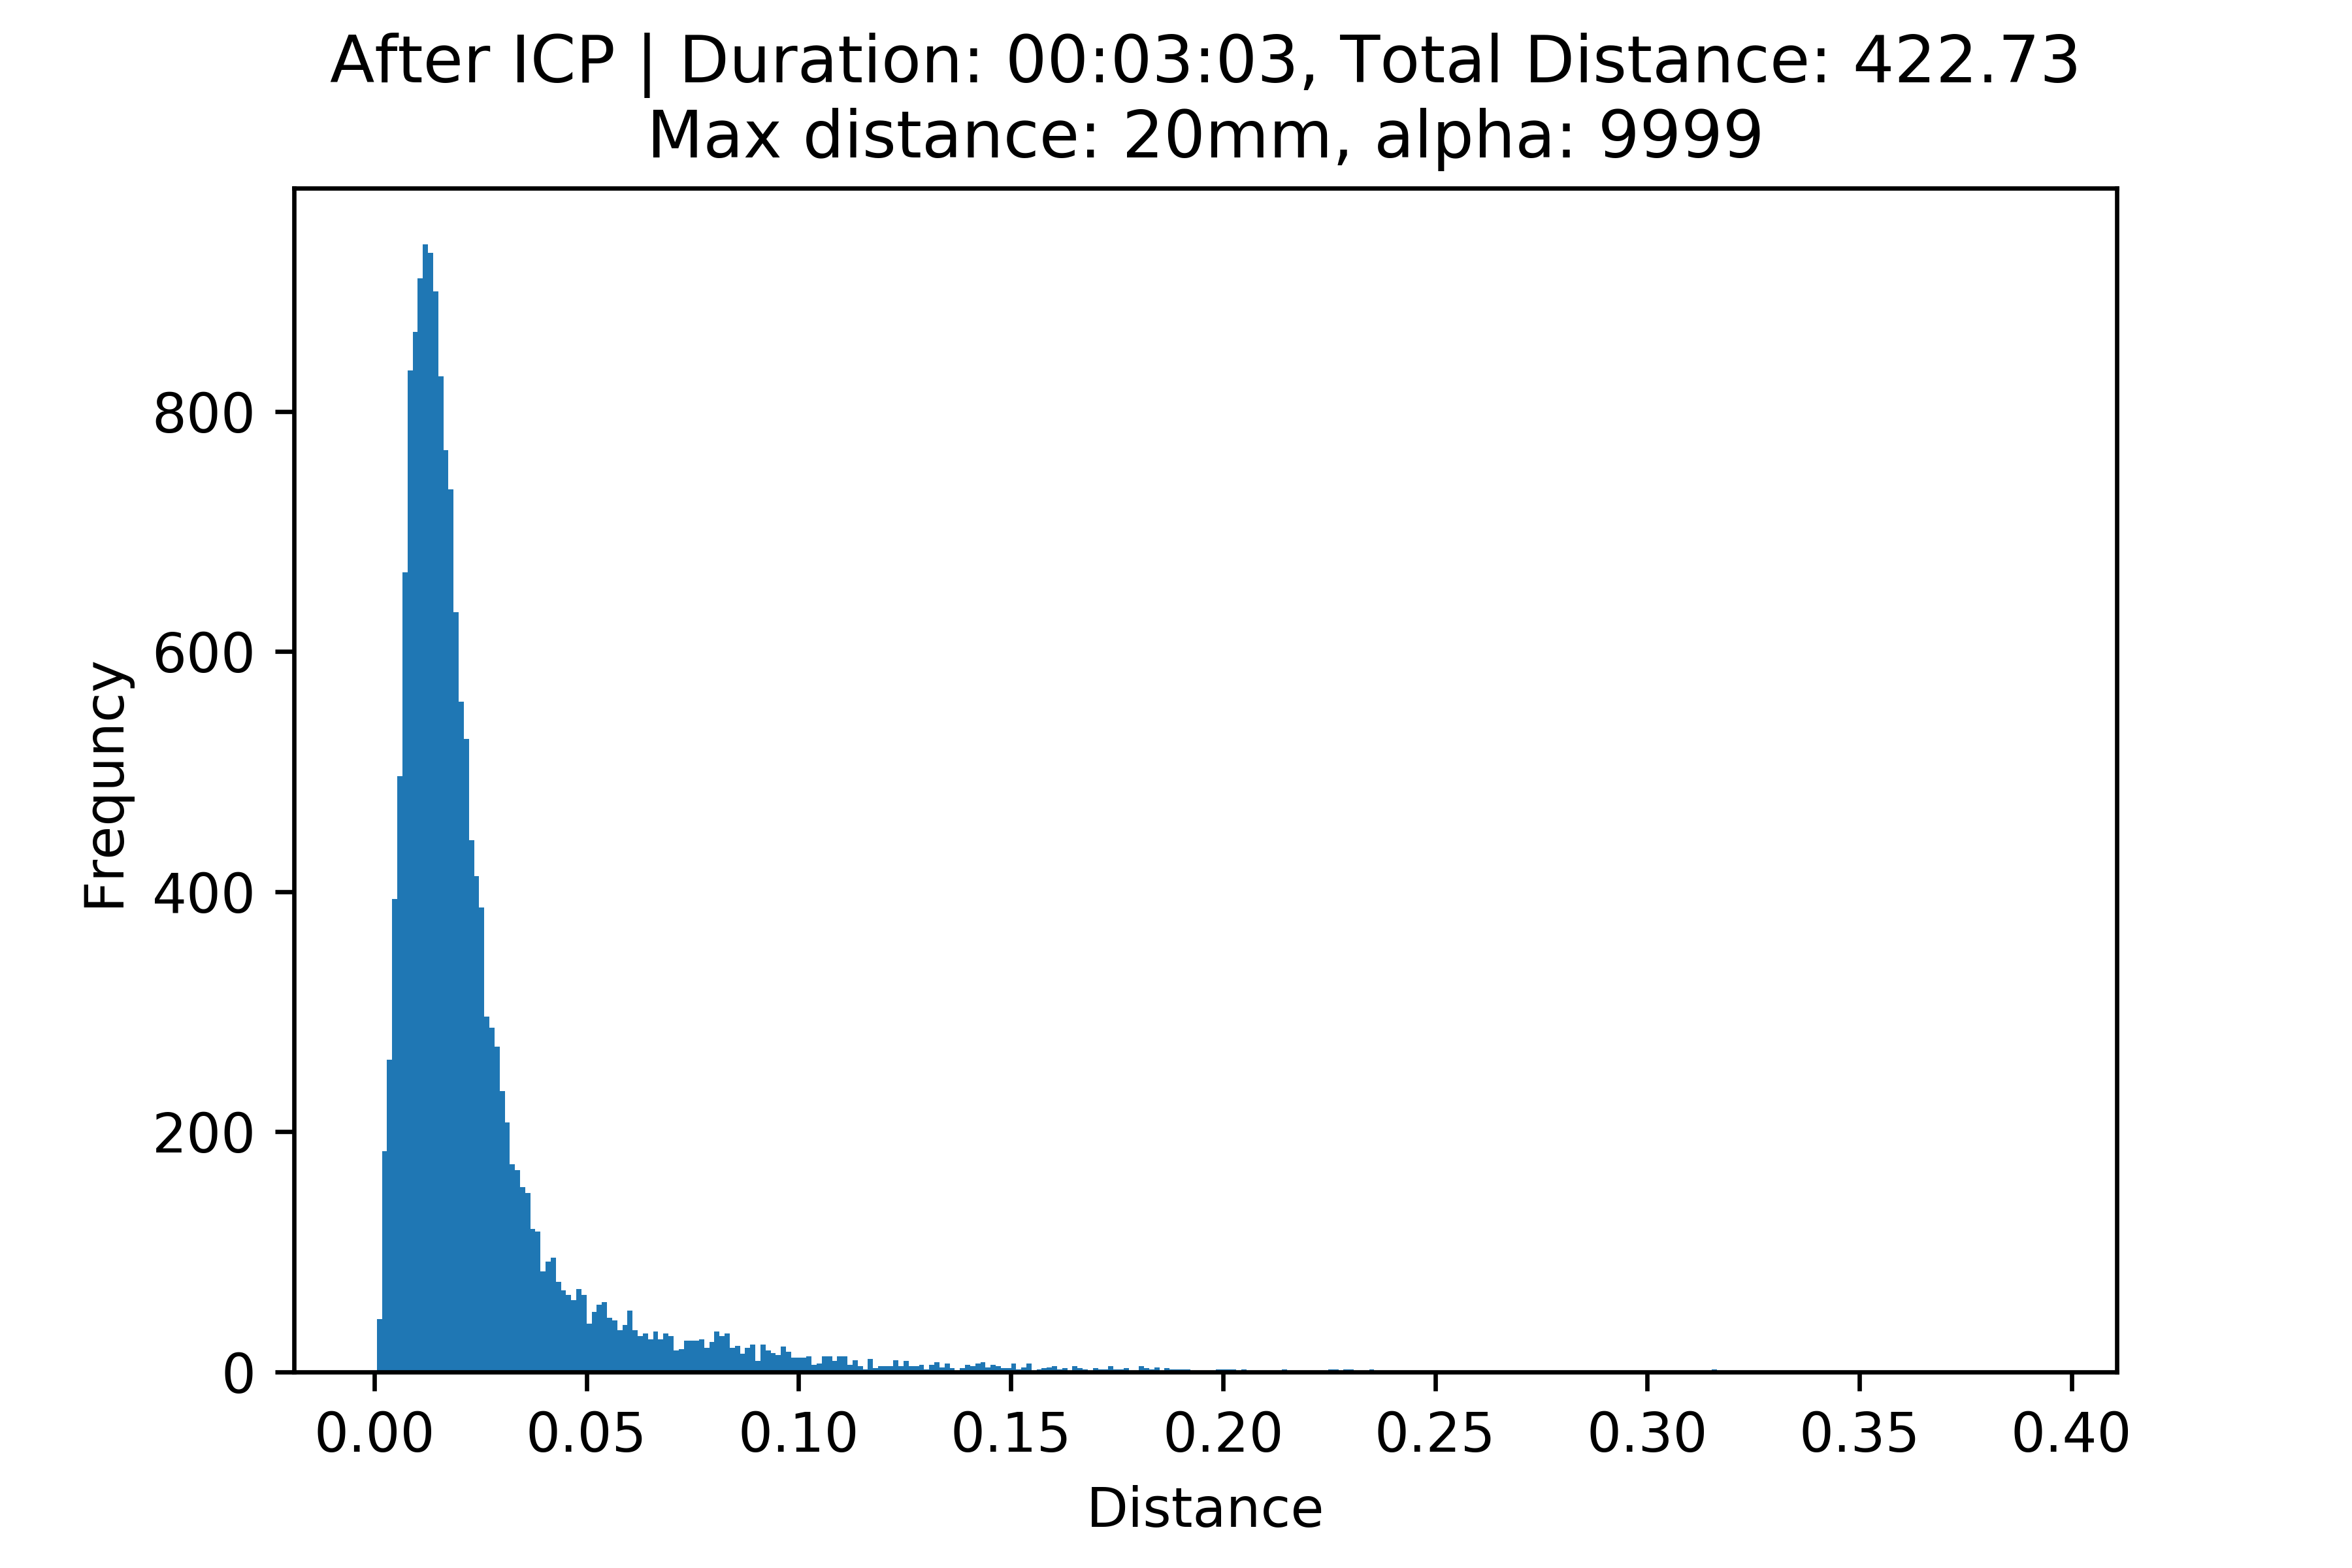
\includegraphics[scale=1]{102_hist_ICP}
\captionsetup{justification=centering}
\caption{The distances histogram after deforming a bundle and aligning it with the original one using ICP}
\label{fig:hist_icp_def}
\end{figure}

% Stoped here last time
 using our tool. by transforming it locally and globally. Essentially, what we mean by local transformation is that we apply different affine transformation matrices for each point in the bundle and local means one affine transformation matrix for all points (no deformation). Then we try to align it again with the original one. We show the results in Figures \ref{fig:hist_original_def} \ref{fig:img_original_def} of local transformation only because it is relatively straightforward for global transformation. The condition value of LSQR we got is 5741672.

\begin{figure}[h!]
\centering
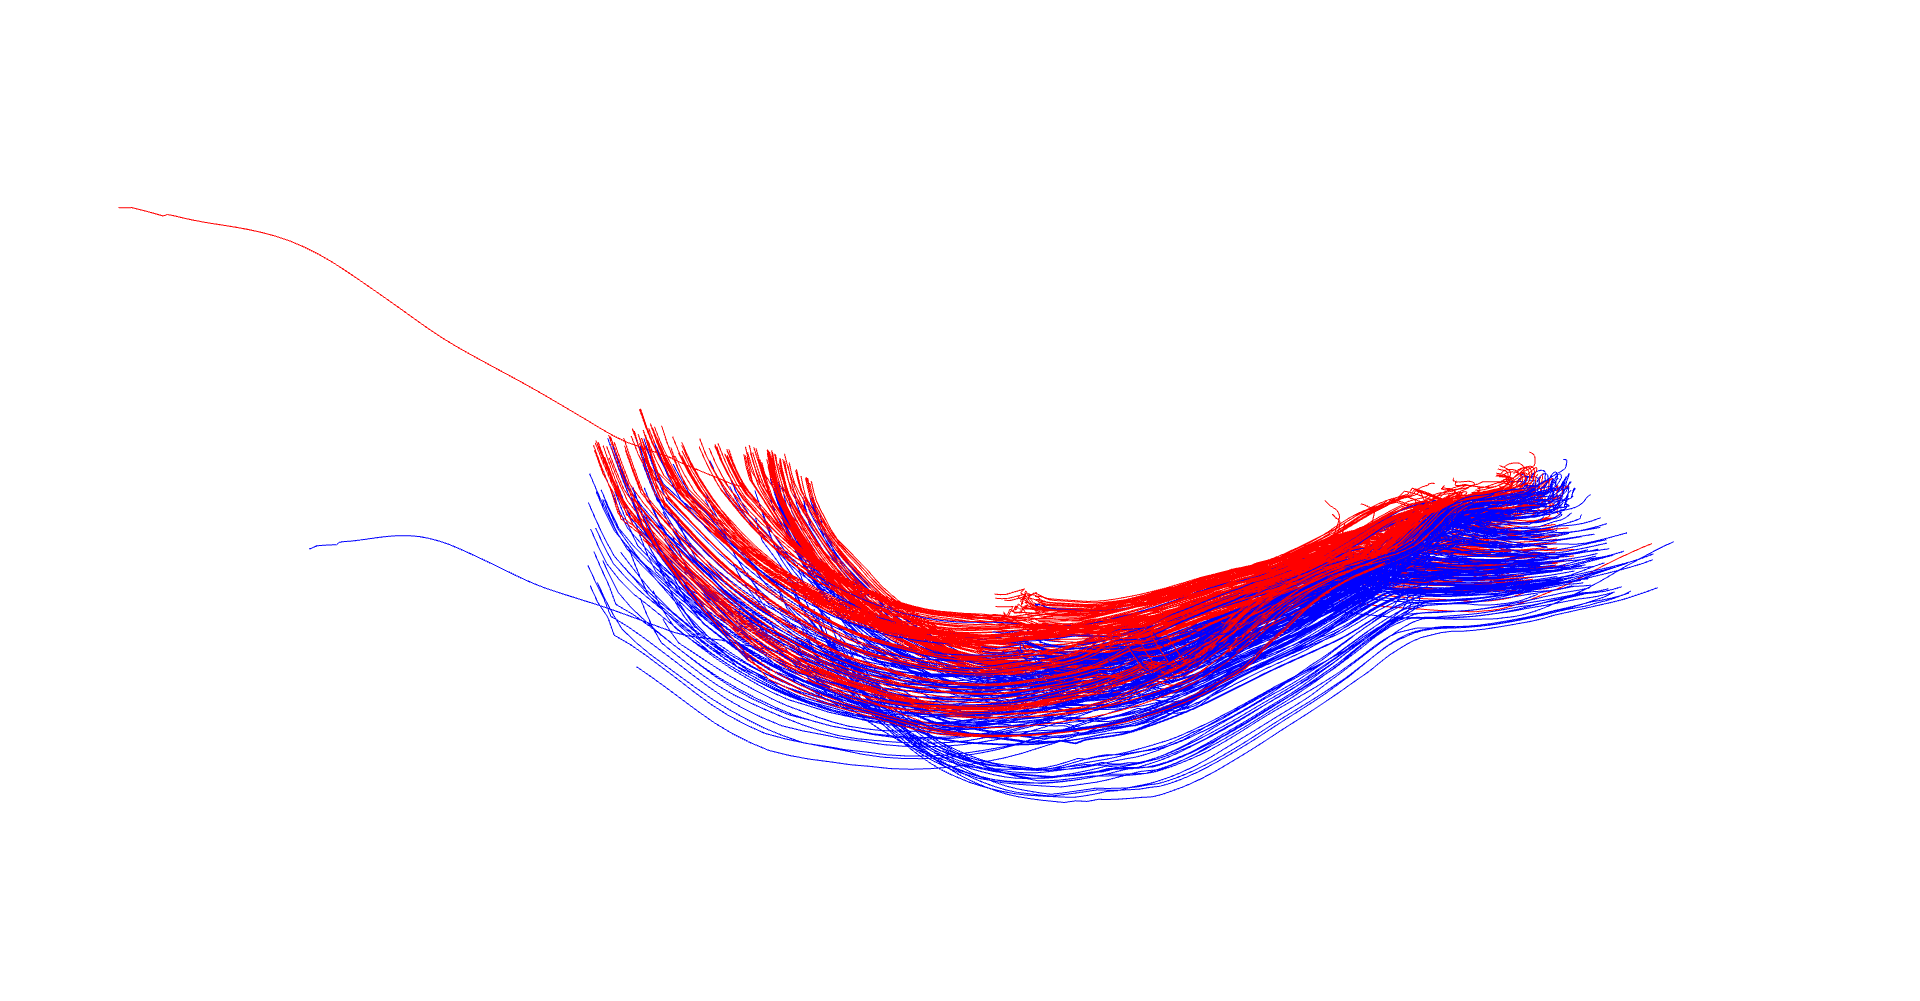
\includegraphics[scale=.3]{102_img_original}
\captionsetup{justification=centering}
\caption{The orientation after deformation}
\label{fig:img_original_def}
\end{figure}
\pagebreak

Next, we align them with DIPY to get the results in Figures \ref{fig:hist_dipy_def} \ref{fig:img_dipy_def}.

\begin{figure}[h!]
\centering
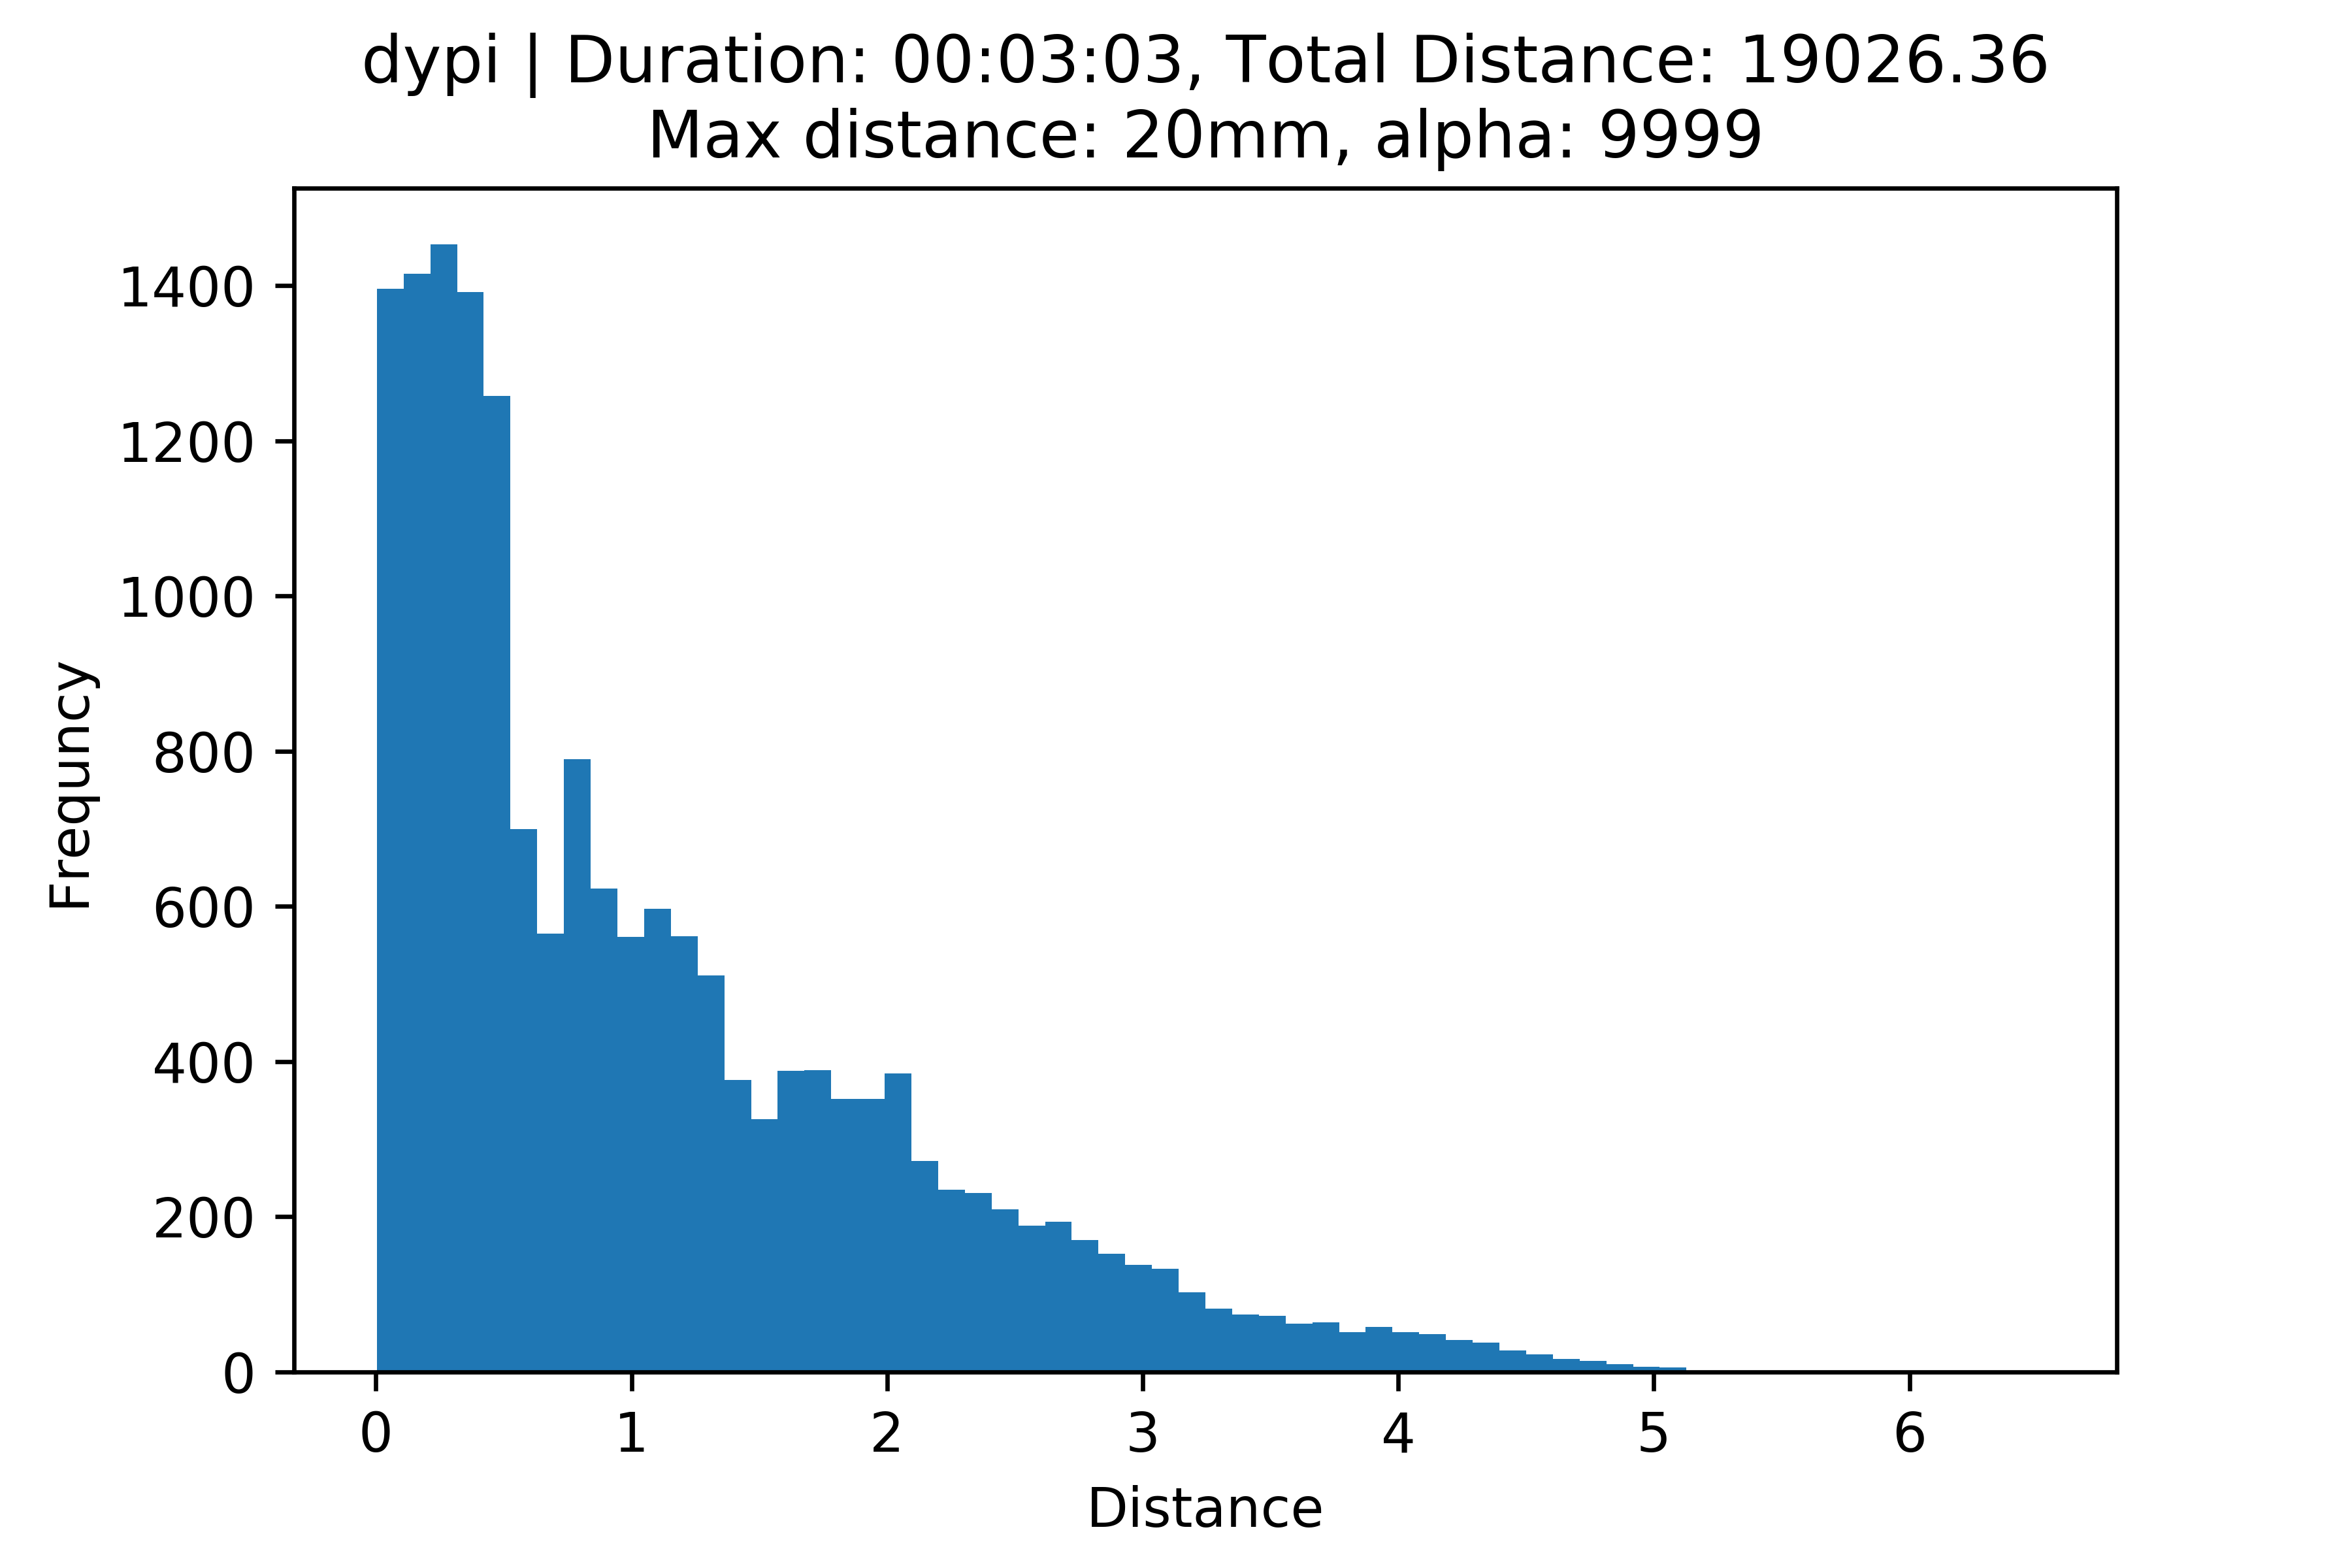
\includegraphics[scale=1]{102_hist_dipy}
\captionsetup{justification=centering}
\caption{The distances histogram after deforming a bundle and aligning it with the original one using DIPY}
\label{fig:hist_dipy_def}
\end{figure}

\begin{figure}[h!]
\centering
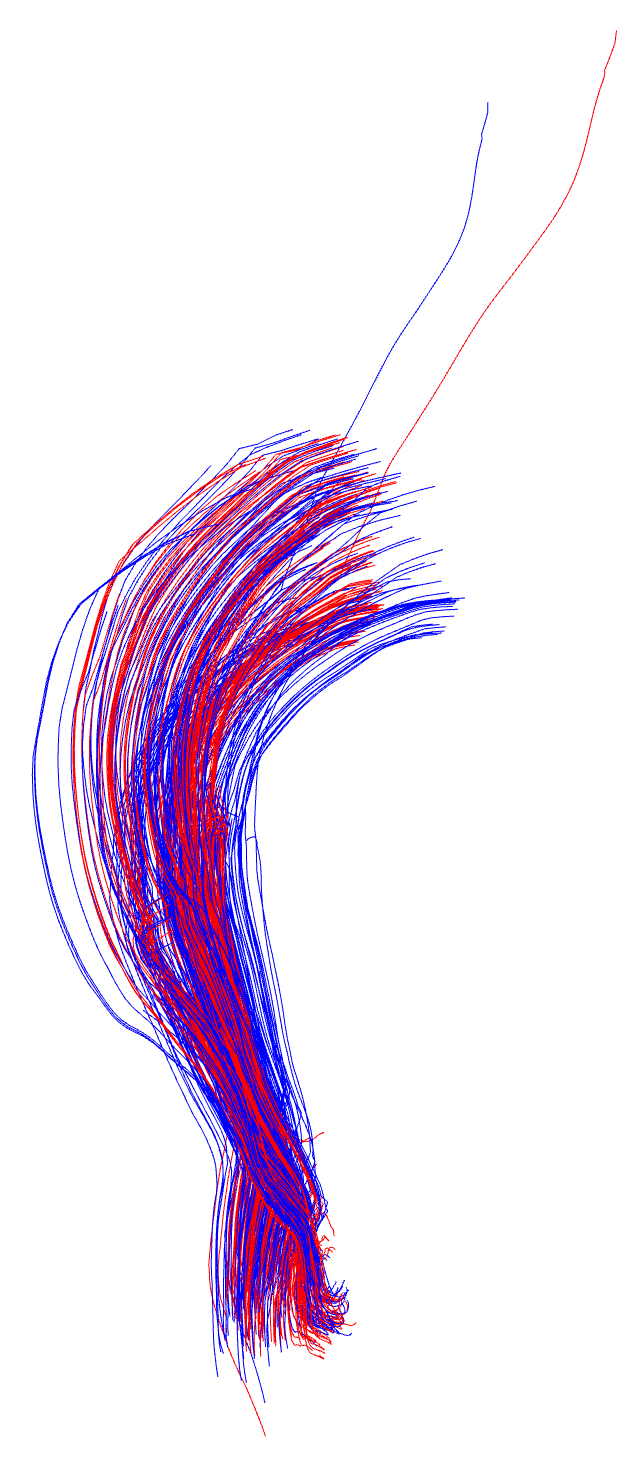
\includegraphics[scale=.3]{102_img_dipy}
\captionsetup{justification=centering}
\caption{The orientation after deforming a bundle and aligning it with the original one using DIPY}
\label{fig:img_dipy_def}
\end{figure}
\pagebreak
We then apply non-rigid ICP registration to get the results in Figures \ref{fig:hist_icp_def} \ref{fig:img_icp_def}.

\begin{figure}[h!]
\centering
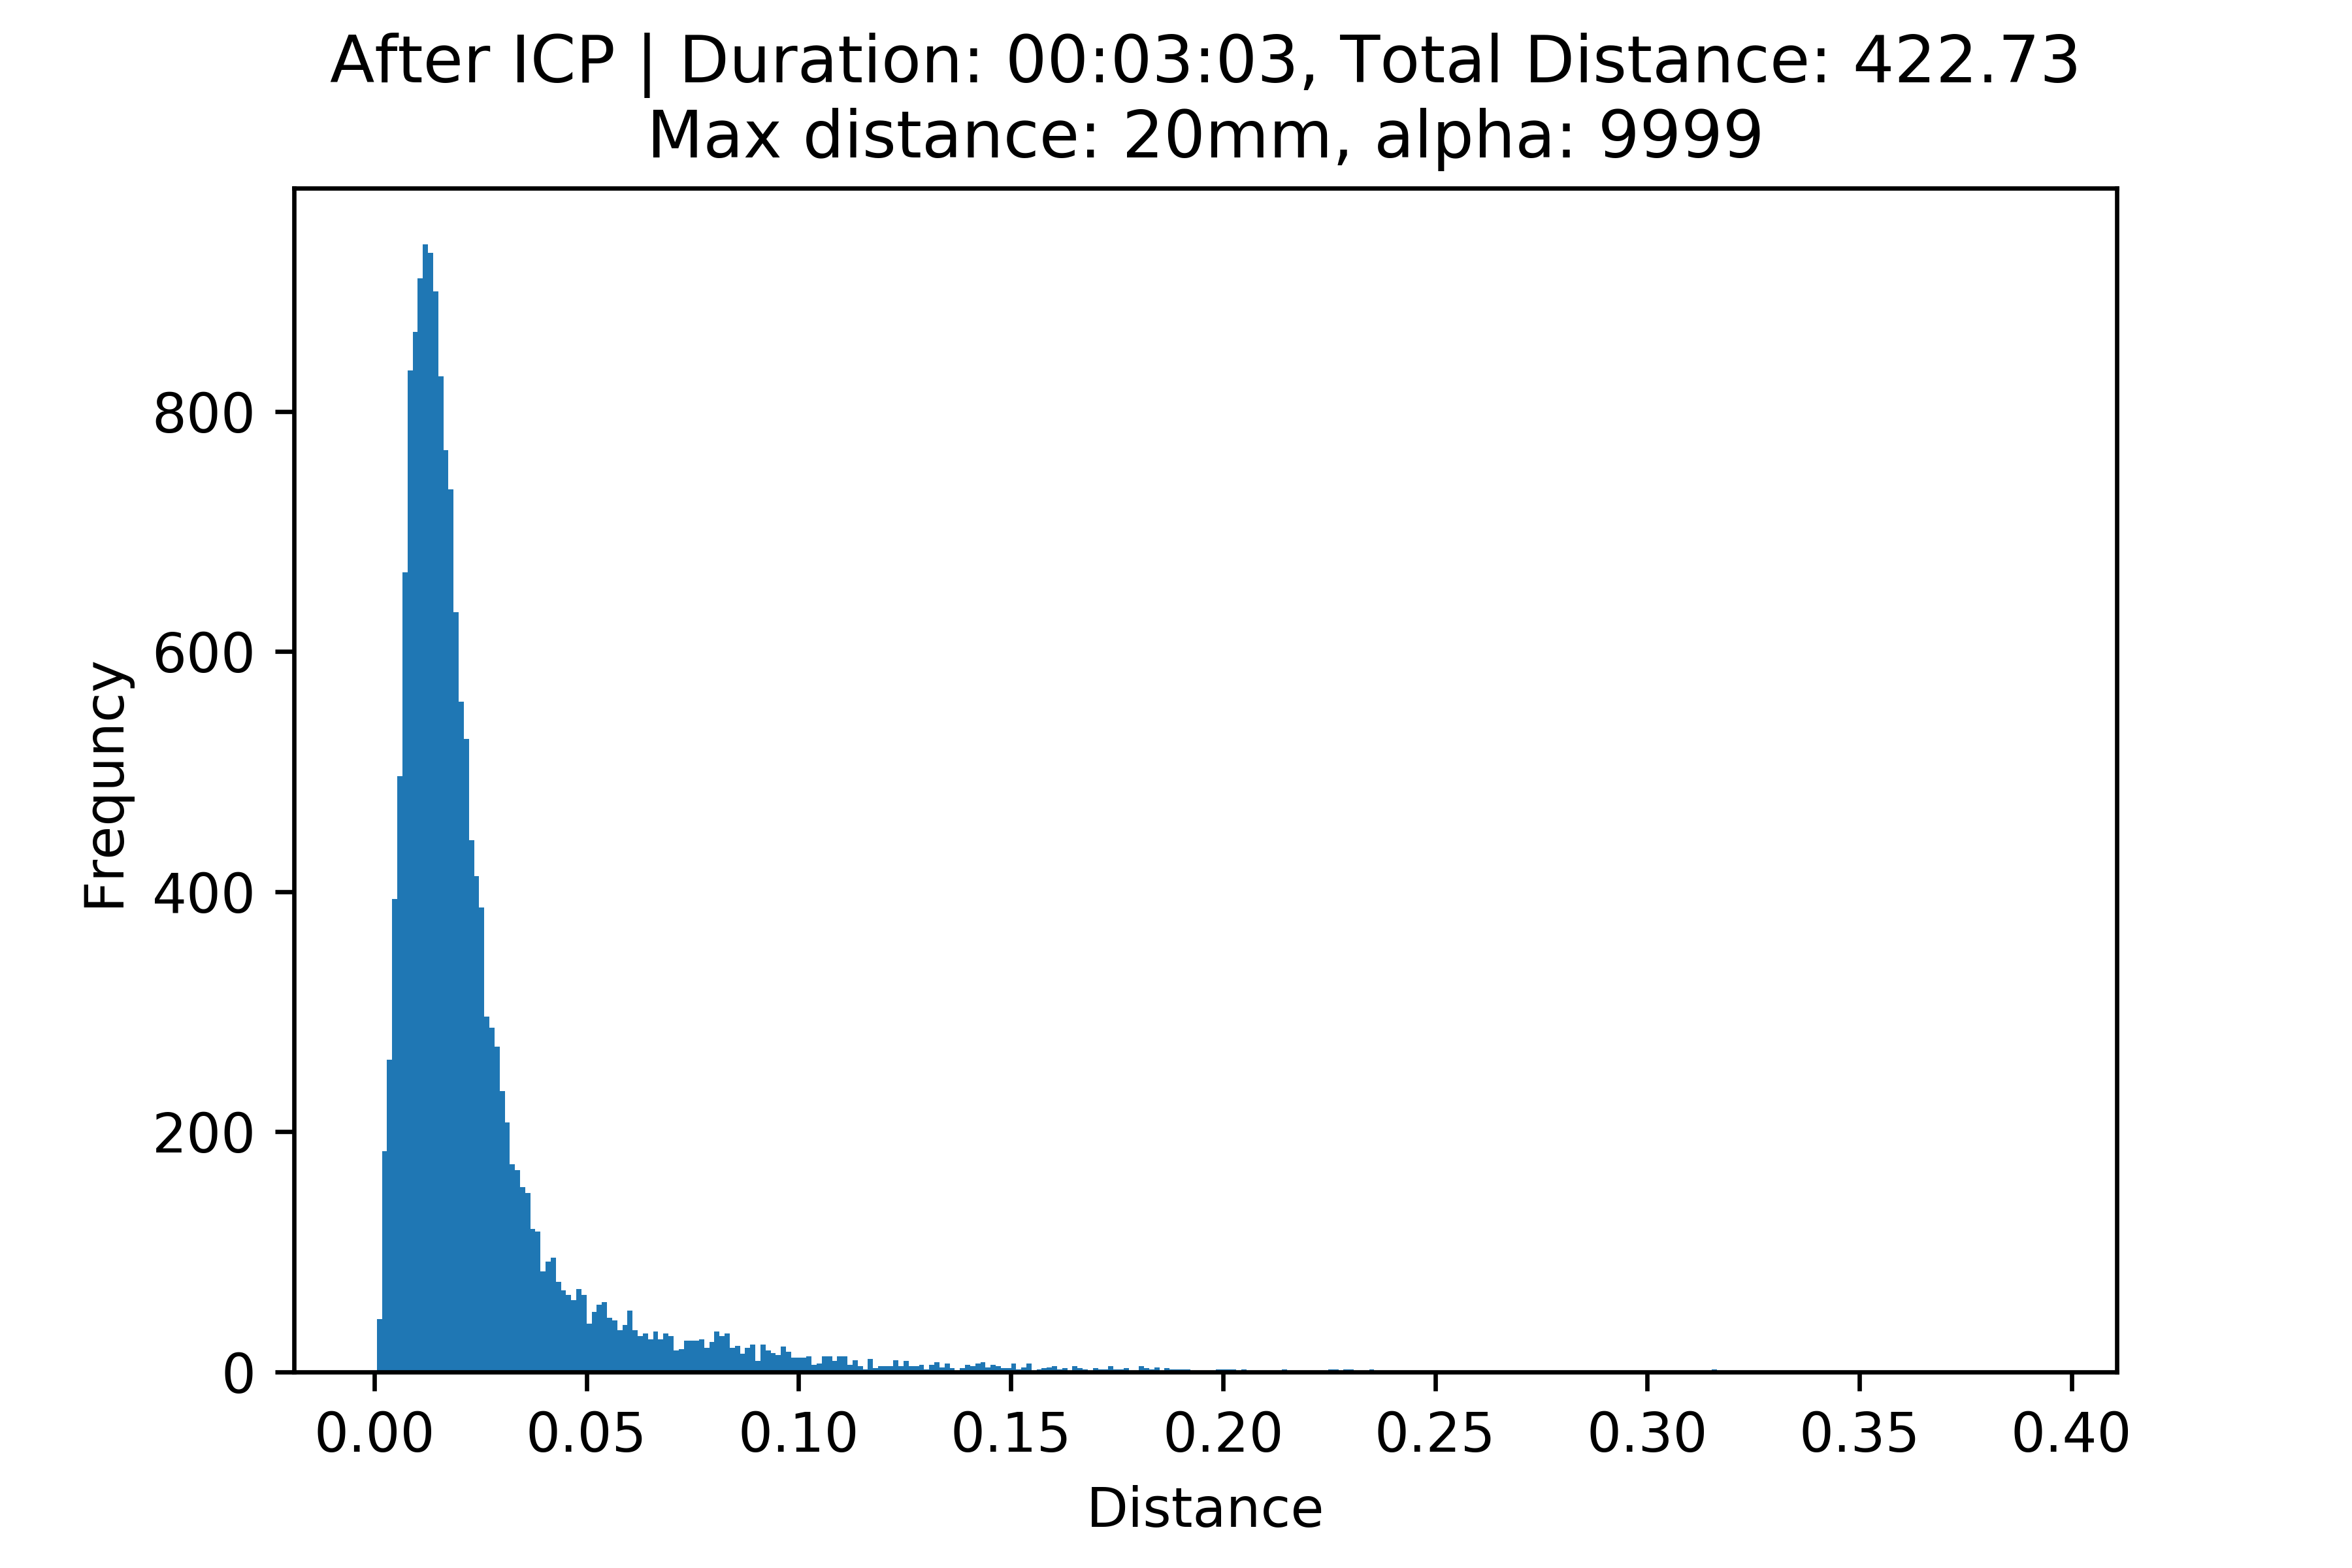
\includegraphics[scale=1]{102_hist_ICP}
\captionsetup{justification=centering}
\caption{The distances histogram after deforming a bundle and aligning it with the original one using ICP}
\label{fig:hist_icp_def}
\end{figure}

\begin{figure}[h!]
\centering
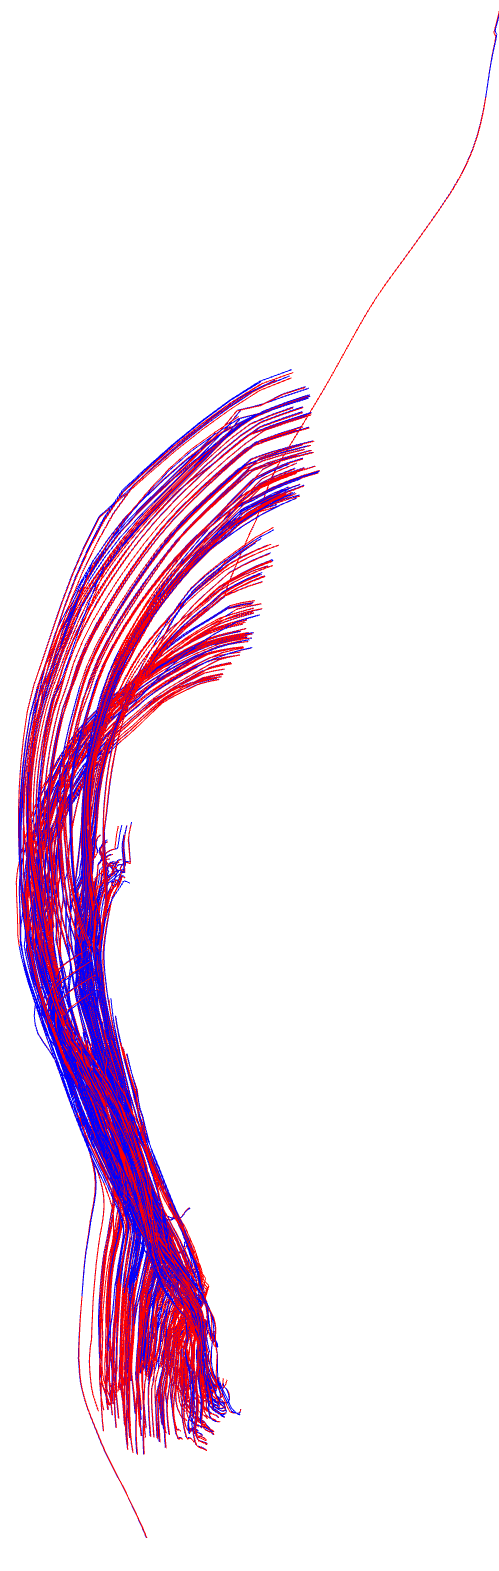
\includegraphics[scale=.3]{102_img_ICP}
\captionsetup{justification=centering}
\caption{The orientation after deforming a bundle and aligning it with the original one using ICP}
\label{fig:img_icp_def}
\end{figure}

\pagebreak

Applying PCA sometimes does not find the right orientation of bundles due to similarity of vertices distribution and that gives similar principle components as shown below:


	\begin{figure}[h!]
	\centering
	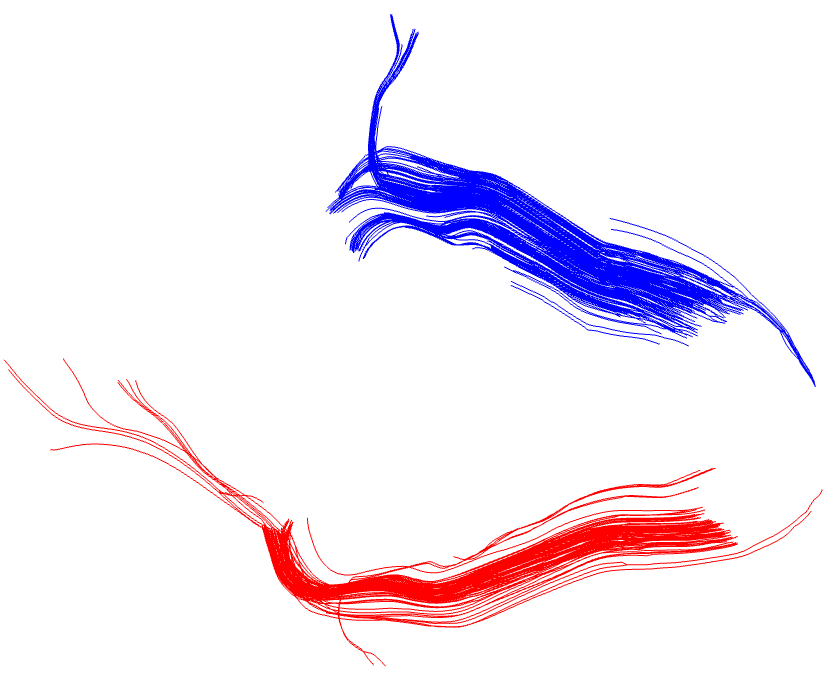
\includegraphics[scale=0.5]{02_img_original}
	\captionsetup{justification=centering}
	\caption{The original coordinate before PCA}
	\label{fig:all_brain}
	\end{figure}
	
	\begin{figure}[h!]
	\centering
	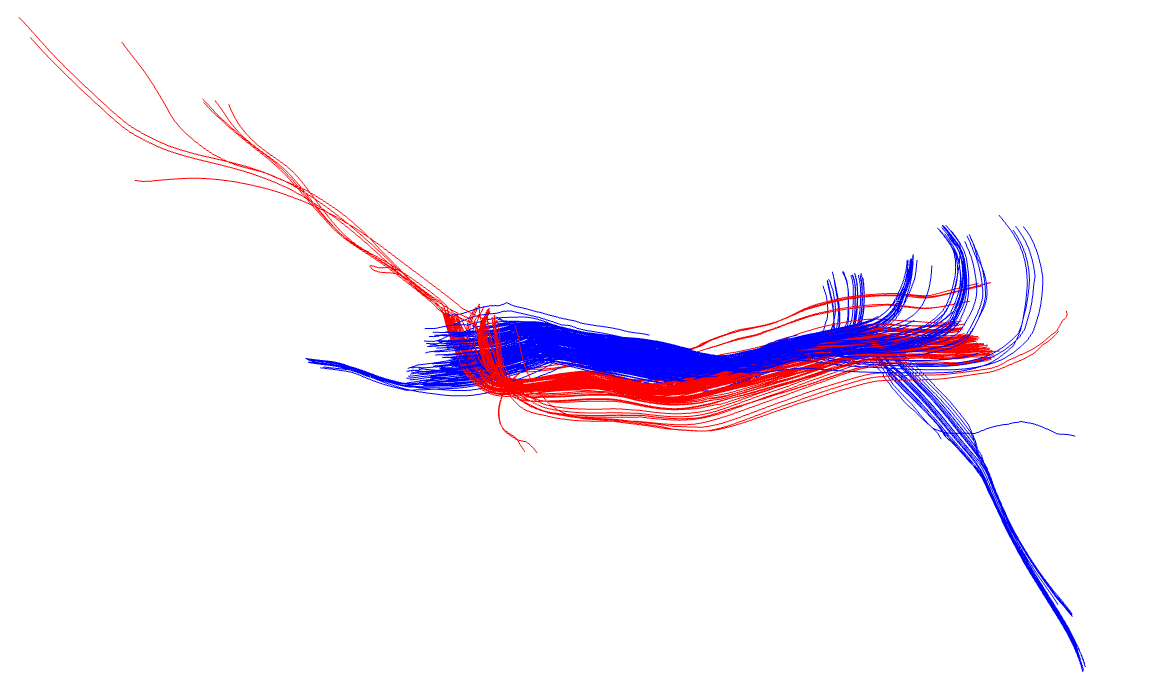
\includegraphics[scale=0.3]{02_img_PCA}
	\captionsetup{justification=centering}
	\caption{The coordinate when PCA fails to find the best alignment}
	\label{fig:all_brain}
	\end{figure}
\pagebreak

Finally, we found that our tool can handle the deformation easily (elastic registration) but \textit{DIPY} can only handle the size by scaling the template bundles.

The \textit{DIPY} method is much faster than our method because it is implemented to reduce the number of points used to calculate the distance. In our test, each tract reduced to 20 points rather than the real number of points as shown in table \{\ref{table:data}\}. Furthermore, as mentioned in \cite{Garyfallidis2012}, \textit{DIPY} uses a minimum average direct-flip distance (MDF) which considers the tract to tract distance whereas our tool considers the point to point distance. To improve our tool, hierarchical clustering bundles can be done and soft membership alignment can be applied.

\end{document}


